\documentclass[12pt,aspectratio=169]{beamer}

% ====================================================
% ====================================================
% USEPACKAGES AND IMPORTS
% ====================================================
% ====================================================

\usepackage[T1]{fontenc}
\usepackage[utf8]{inputenc}
\usepackage[english]{babel}

% tables
\usepackage{tabularx}
\usepackage{colortbl}
\usepackage{multirow}
\usepackage{makecell}

% tikz and colors
\usepackage{tikz}
\usepackage{xcolor}
\usepackage{pgfplots}
\usepackage{pgfplotstable}
\usepackage{tikzsymbols}

\usetikzlibrary{calc}
\usetikzlibrary{trees}
\usetikzlibrary{patterns}
\usetikzlibrary{shadings}
\usetikzlibrary{positioning}
\usetikzlibrary{intersections}
\usepgfplotslibrary{patchplots}
\usepgfplotslibrary{fillbetween}
\usetikzlibrary{decorations.pathreplacing}

\usetikzlibrary{arrows}
\usetikzlibrary{arrows.meta}

\usetikzlibrary{shapes}
\usetikzlibrary{shapes.arrows}
\usetikzlibrary{shapes.callouts}
\usetikzlibrary{shapes.symbols}
\usetikzlibrary{shapes.geometric}

% boxes
\usepackage[many]{tcolorbox}

% math packages and fonts
\usepackage{bm}
\usepackage{ccfonts}
\usepackage{eulervm}
\usepackage{amsmath}
\usepackage{amsfonts}
\usepackage{amssymb}
\usepackage{amsthm}
\usepackage{mathtools}
\usepackage{nicefrac}
\usepackage{slashed}
\usepackage{bbold}
\usepackage{array}
\usepackage{cancel}

% algorithms and listings
\usepackage[ruled,vlined,linesnumbered]{algorithm2e}
\usepackage{listings}
\usepackage{setspace}

\tcbuselibrary{listings}
\tcbuselibrary{breakable}
\tcbuselibrary{skins}

% misc
\usepackage{soul}
\usepackage{pifont}
\usepackage{skull}
\usepackage{multicol}
\usepackage{animate}
\usepackage{hyperref}
\usepackage{wasysym}
\usepackage[absolute,overlay]{textpos}
\usepackage[hang,flushmargin]{footmisc}

% ====================================================
% ====================================================
% LAYOUT AND THEME
% ====================================================
% ====================================================

\usetheme{Copenhagen}

% color definitions
\definecolor{myblue1}{RGB}{35,119,189}
\definecolor{myblue2}{RGB}{95,179,238}
\definecolor{myblue3}{RGB}{129,168,207}
\definecolor{myblue4}{RGB}{26,89,142}

\definecolor{myred1}{RGB}{247,12,12}

% set theme colors
\setbeamercolor*{structure}{fg=myblue1,bg=blue}
\setbeamercolor*{palette primary}{use=structure,fg=white,bg=structure.fg}
\setbeamercolor*{palette secondary}{use=structure,fg=white,bg=structure.fg!75!black}
\setbeamercolor*{palette tertiary}{use=structure,fg=white,bg=structure.fg!50!black}
\setbeamercolor*{palette quaternary}{fg=black,bg=white}

\setbeamertemplate{itemize item}[circle]
\setbeamertemplate{itemize subitem}[circle]
\setbeamertemplate{itemize subsubitem}[circle]

\setbeamertemplate{enumerate item}[circle]
\setbeamertemplate{enumerate subitem}[circle]
\setbeamertemplate{enumerate subsubitem}[circle]

\setbeamercolor{itemize item}{fg=myblue1}
\setbeamercolor{itemize subitem}{fg=myblue1}
\setbeamercolor{itemize subsubitem}{fg=myblue1}

\setbeamertemplate{section in toc}[circle]
\setbeamertemplate{subsection in toc}[circle]
\setbeamerfont{subsection in toc}{size=\scriptsize}

\setbeamercolor{frametitle continuation}{fg=black}

% title graphic -- sap logo and dhbw logo
\titlegraphic{
\includegraphics[scale=0.1]{../03_img/logo_sap}\hspace*{4.75cm}~%
   	
\includegraphics[scale=0.05]{../03_img/logo_dhbw}
}

\makeatletter
% frame title
\defbeamertemplate*{frametitle}{mydefault}[1][left]
{
  	\ifbeamercolorempty[bg]{frametitle}{}{\nointerlineskip}%
  	\nointerlineskip%
 	\@tempdima=\textwidth%
  	\advance\@tempdima by\beamer@leftmargin%
  	\advance\@tempdima by\beamer@rightmargin%
  	\begin{tcolorbox}[
  		enhanced,
  		outer arc=0pt,
  		arc=0pt,
  		boxrule=0pt,
  		top=0pt,
  		bottom=0pt,
  		enlarge left by=-\beamer@leftmargin,
  		enlarge right by=-\beamer@rightmargin,
  		width=\paperwidth,
  		nobeforeafter,
  		interior style={
    			left color=myblue2,
    			right color=white
    		},
  		shadow={0mm}{-0.4mm}{0mm}{black!60,opacity=0.6},    
  		shadow={0mm}{-0.8mm}{0mm}{black!40,opacity=0.4},    
  	]
    	\usebeamerfont{frametitle}%
    	\vbox{}\vskip-1ex%
    	\if@tempswa\else\csname beamer@fte#1\endcsname\fi%
    	\insertframetitle\par%
    	{%
      		\ifx\insertframesubtitle\@empty%
      		\else%
      		{\usebeamerfont{framesubtitle}\usebeamercolor[fg]{black}\insertframesubtitle\strut\par}%
      		\fi
    	}%
    	\vskip-1ex%
    	\if@tempswa\else\vskip-.3cm\fi
  	\end{tcolorbox}%
}

% footline of a frame
\defbeamertemplate*{footline}{mysplit theme}
{%
  	\leavevmode%
  	\hbox{
		\begin{beamercolorbox}[
			wd=.5\paperwidth,ht=2.5ex,dp=1.125ex,leftskip=.3cm plus1fill,rightskip=.3cm
		]{author in head/foot}%
    			\usebeamerfont{author in head/foot}\insertshortauthor\ (\insertinstitute), \insertdate
  		\end{beamercolorbox}%
  		\begin{beamercolorbox}[
			wd=.5\paperwidth,ht=2.5ex,dp=1.125ex,leftskip=.3cm,rightskip=.3cm plus1fil
		]{title in head/foot}%
    			\usebeamerfont{title in head/foot}\insertshorttitle\hfill
    			\insertprefix-\insertframenumber/\inserttotalframenumber\hspace*{0.5em}
  		\end{beamercolorbox}}%
  	\vskip0pt%
}
\makeatother

% ====================================================
% ====================================================
% COMMANDS AND GENERAL DEFINITIONS
% ====================================================
% ====================================================

% page number prefix
\newcommand\insertprefix{}  % empty by default
\newcommand\prefix[1]{\renewcommand\insertprefix{#1}}

% math definitions
% ====================================================
\DeclareMathOperator*{\argmax}{arg\,max}
\DeclareMathOperator*{\argmin}{arg\,min}
\newcommand*\diff{\mathop{}\!\mathrm{d}}

\newcommand*{\vertbar}{\rule[-1ex]{0.5pt}{2.5ex}}
\newcommand*{\horzbar}{\rule[.5ex]{2.5ex}{0.5pt}}

% commands
% ====================================================

% highlight commands
% --------------------------------------------------------------------------------------------------------
% highlight command
\newcommand{\highlight}[1]{\textcolor{myblue1}{\textbf{#1}}}
\newcommand{\highlighttt}[1]{\textcolor{myblue1}{\texttt{#1}}}
\newcommand{\Highlight}[1]{\textcolor{myred1}{\textbf{#1}}}

% blue color boxes (with frame/without frame/without fill)
\newtcolorbox{boxBlue}{colback=myblue1!10!white,colframe=myblue4}
\newtcolorbox{boxBlueNoFrame}{colback=myblue1!10!white,colframe=myblue1!10!white}
\newtcolorbox{boxBlueNoFill}{colback=white,colframe=myblue4}

% font commands
% --------------------------------------------------------------------------------------------------------
\newcommand{\linkstyle}[1]{\underline{\smash{\texttt{#1}}}} 		% style of hyperlinks

% tikz commands
% --------------------------------------------------------------------------------------------------------

% yellow sticky note
\newcommand{\bubble}[3]{
\begin{textblock}{100}(#1, #2)
      	\begin{tikzpicture}
		\node[rectangle,draw=yellow,very thick,fill=yellow!60,align=center] at (0,0) {#3};
	\end{tikzpicture}
\end{textblock}
}

\newcommand{\floattext}[3]{
\begin{textblock}{100}(#1, #2)
      	#3
\end{textblock}
}

\newcommand{\doublecircle}[2]{
	\draw[fill=white,draw=myblue1] (#1,#2) circle (2mm);
	\draw[fill=myblue1,draw=myblue1] (#1,#2) circle (1.5mm);
}

% slide modifiers
% --------------------------------------------------------------------------------------------------------
% mark slide as optional
\newcommand{\optional}{
	\begin{textblock}{100}(0.15,0.30)
      		
\includegraphics[scale=0.2]{../03_img/scream}
    	\end{textblock}
}

% mark slide as important
\newcommand{\important}{
	\begin{textblock}{100}(0.10,0.15)
      		
\includegraphics[scale=0.1]{../03_img/important}
    	\end{textblock}
}

% citation
% --------------------------------------------------------------------------------------------------------
% first argument in {book, online, article}
\newcommand{\literature}[5]{
	\setbeamertemplate{bibliography item}[#1]
	\bibitem{#2}
	\highlight{#3} \\
	\textcolor{darkgray}{\textit{#4}} \\
	\textcolor{black}{#5}
}
% cite content
\newcommand{\citeAuthor}[3]{\vfill\scriptsize\textcolor{lightgray}{#1 \cite{#2} #3}}

% slide architecture
% --------------------------------------------------------------------------------------------------------
% divide frame into two parts
\newcommand{\divideTwo}[4]{
	\begin{minipage}{#1\textwidth}
		#2
	\end{minipage}
	\hfill
	\begin{minipage}{#3\textwidth}
		#4
	\end{minipage}
}

% divide frame into two parts (start on top)
\newcommand{\divideTwoTop}[4]{
	\begin{minipage}[t]{#1\textwidth}
		#2
	\end{minipage}
	\hfill
	\begin{minipage}[t]{#3\textwidth}
		#4
	\end{minipage}
}

% special pages
% --------------------------------------------------------------------------------------------------------
% title page
\newcommand{\maketitlepage}{
	{
		\beamertemplatenavigationsymbolsempty
		\usebackgroundtemplate{%
			\tikz[overlay,remember picture] \node[opacity=0.2, at=(current page.center)] {
  				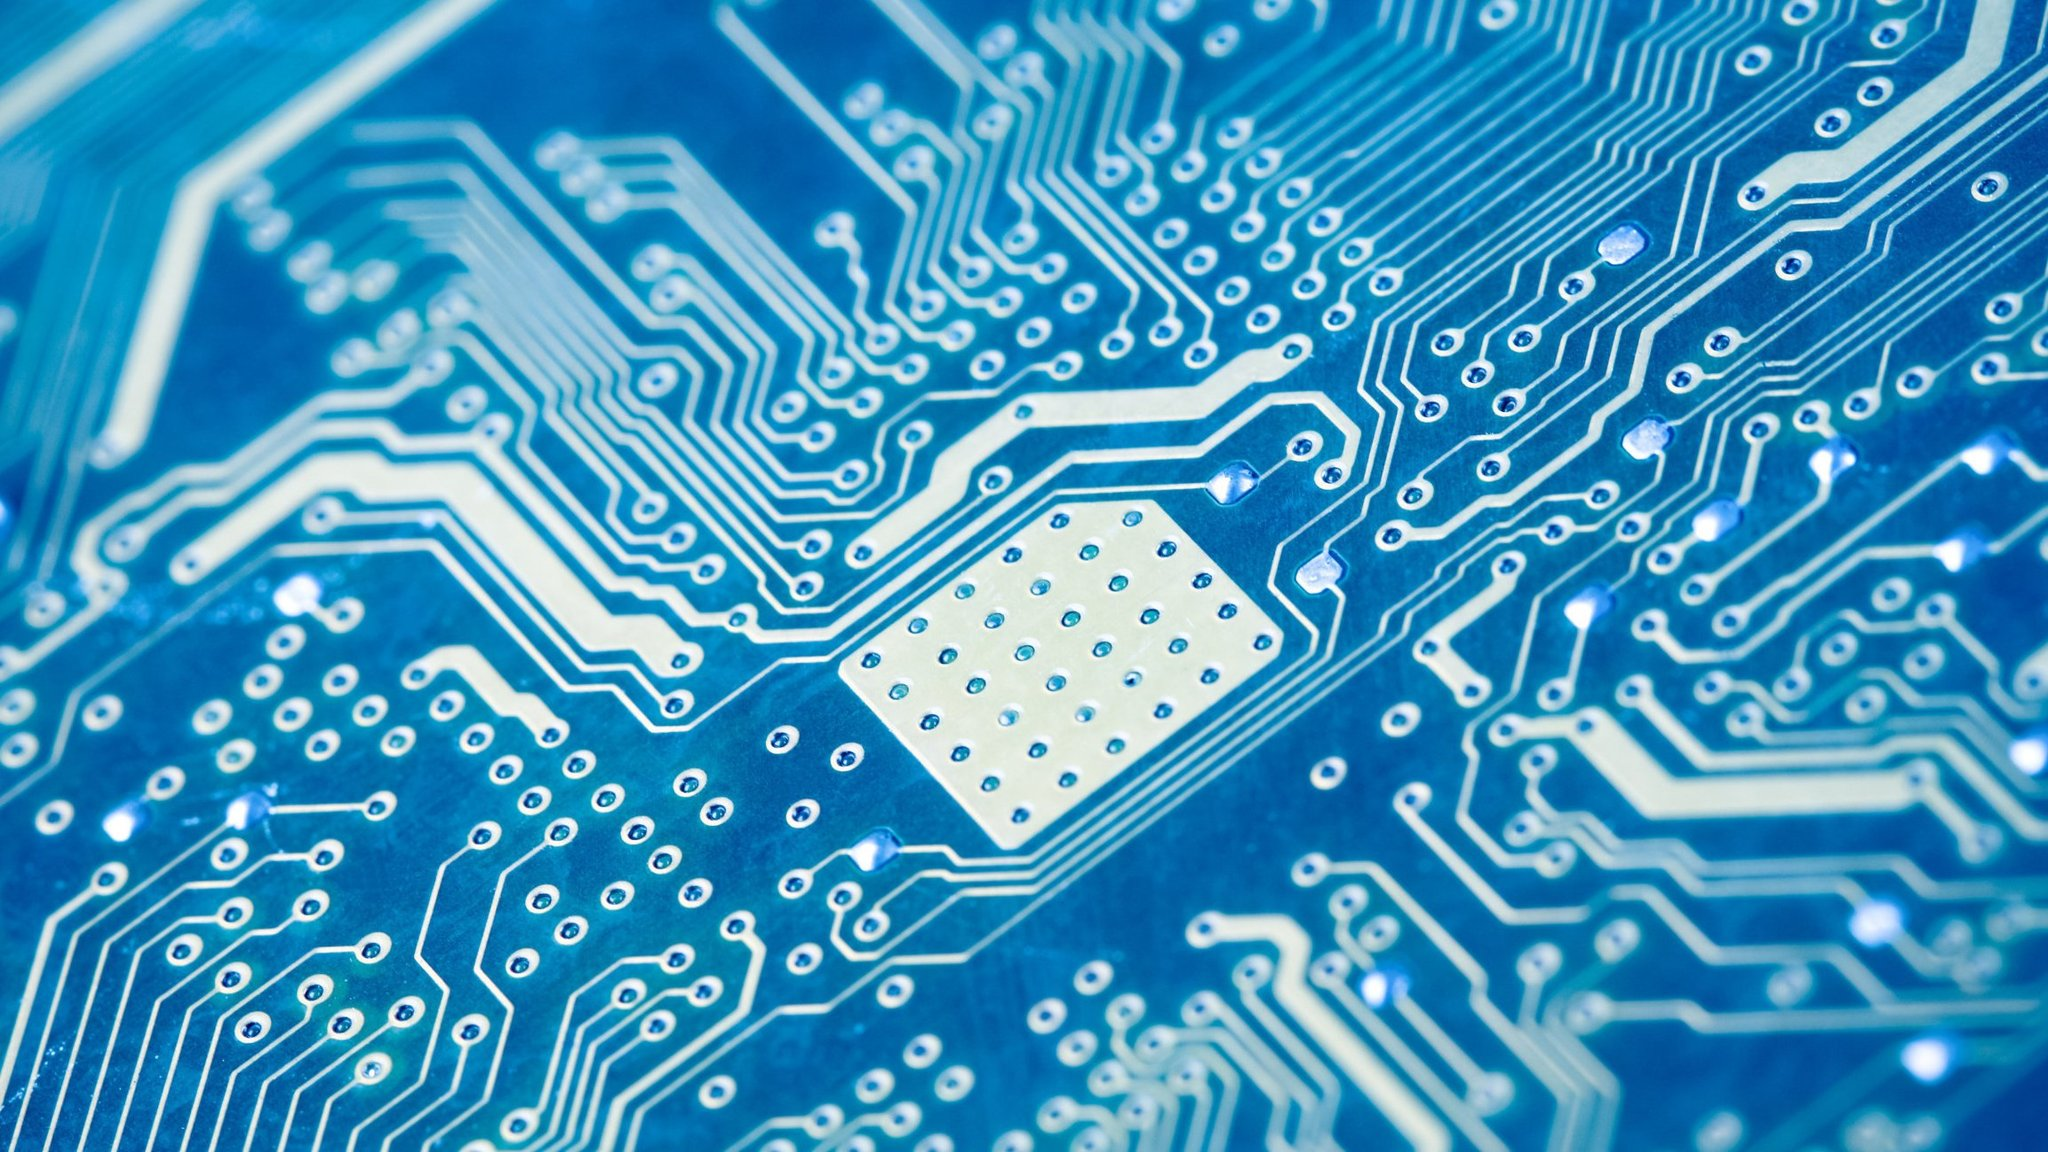
\includegraphics[height=\paperheight,width=\paperwidth]{../03_img/processor.jpg}
			};
		}
		\begin{frame}[plain]
			\vspace*{0.75cm}
			\maketitle
			\vfill
			\begin{center}
				\footnotesize Find all slides on \href{https://github.com/DaWe1992/Applied_ML_Fundamentals}{\linkstyle{GitHub}}
			\end{center}
		\end{frame}
	}
}

% divider page
\newcommand{\makedivider}[1]{
	{
		\beamertemplatenavigationsymbolsempty
		\usebackgroundtemplate{%
			\tikz[overlay,remember picture] \node[opacity=0.2, at=(current page.center)] {
  				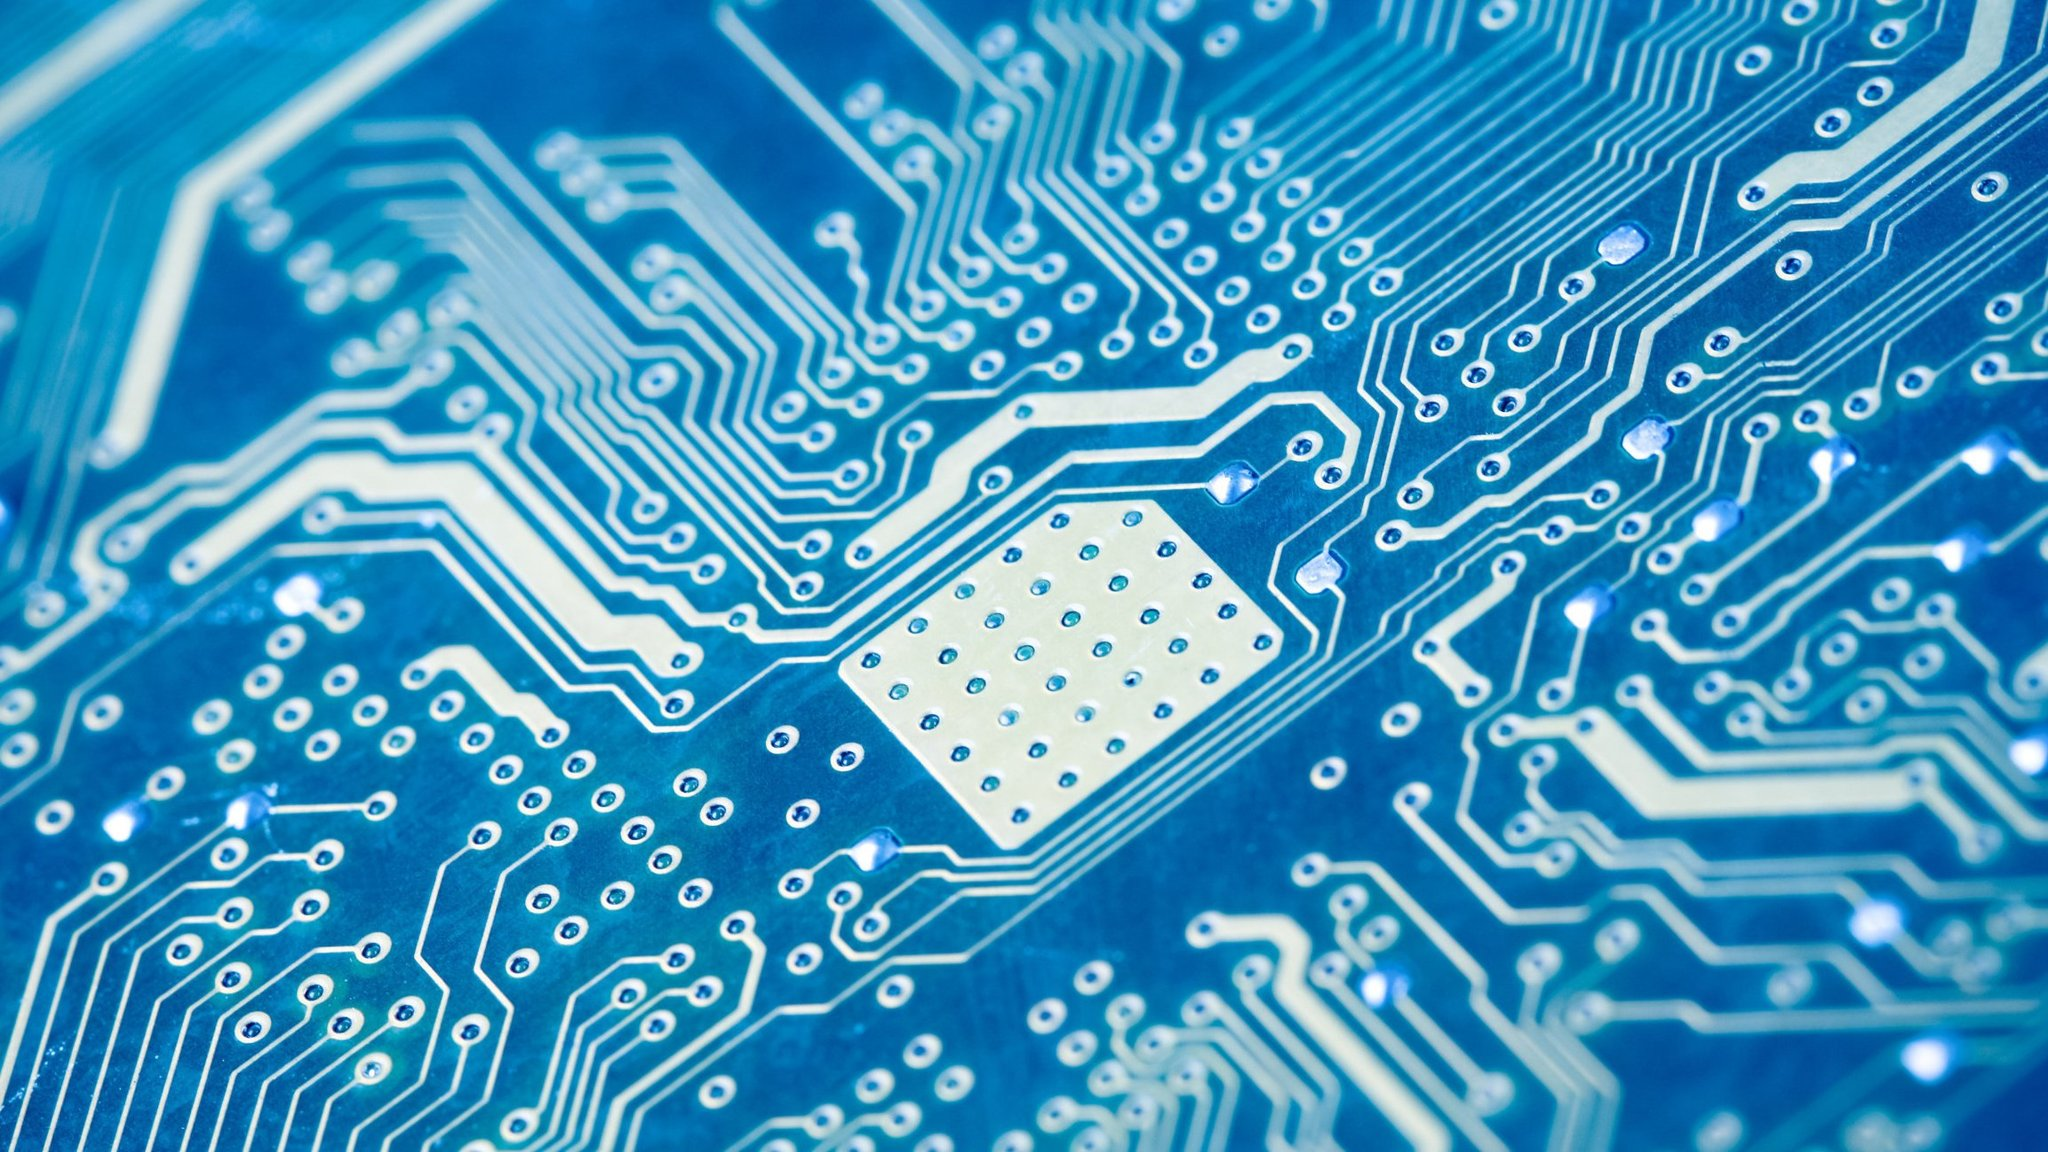
\includegraphics[height=\paperheight,width=\paperwidth]{../03_img/processor.jpg}
			};
		}
		\begin{frame}[plain]
			\vfill
			\begin{boxBlue}
				\centering
				\textbf{Section:} \\
				\large \highlight{#1}
			\end{boxBlue}
			\vfill
			\centering
			
\includegraphics[scale=0.05]{../03_img/logo_dhbw.png}
			\vfill
		\end{frame}
	}
}

% overview page
\newcommand{\makeoverview}[1]{
	\begin{frame}{Lecture Overview}{}
		\begin{tabbing}
			\hspace*{3.5cm}\= \kill
			\ifnum #1=1 \highlight{\textbf{Unit I:}} \else \textbf{Unit I:} \fi
			\> \ifnum #1=1 \highlight{Machine Learning Introduction} \else Machine Learning Introduction \fi \\
		\end{tabbing}
	\end{frame}
}

% thank you page
\newcommand{\makethanks}{
	{\beamertemplatenavigationsymbolsempty
	\begin{frame}[plain]
		\vfill
		\begin{boxBlue}
			\centering
			\Large \highlight{Thank you very much for the attention!}
		\end{boxBlue}
		
		\vfill\footnotesize
		\begin{tabbing}
			\hspace*{1.5cm}\= \kill
			\highlight{Topic:} 	\> \inserttitle \\
			\highlight{Date:} 	\> \insertdate
		\end{tabbing}
		
		\vfill
		\highlight{Contact:} \\
		\insertauthor\ (D062271) \\
		\insertinstitute \\
		\href{mailto:daniel.wehner@sap.com}{\linkstyle{daniel.wehner@sap.com}}
		
		\vfill\normalsize
		\begin{center}
			\large\highlight{Do you have any questions?}
		\end{center}
		\vfill
	\end{frame}}
}

% global pfgplots settings
% --------------------------------------------------------------------------------------------------------
\pgfplotsset{
	% allow filtering of data for pgfplots
	discard if/.style 2 args={
        		x filter/.code={
            		\edef\tempa{\thisrow{#1}}
            		\edef\tempb{#2}
            		\ifx\tempa\tempb
                		\def\pgfmathresult{inf}
            		\fi
        		}
    	},
    	discard if not/.style 2 args={
        		x filter/.code={
            		\edef\tempa{\thisrow{#1}}
            		\edef\tempb{#2}
            		\ifx\tempa\tempb
            		\else
                		\def\pgfmathresult{inf}
            		\fi
        		}
    	}
}


% ====================================================
% ====================================================
% PRESENTATION DATA
% ====================================================
% ====================================================

\title[Deep Learning]{*** Applied Machine Learning Fundamentals *** Neural Networks / Deep Learning}
\institute{SAP\,SE}
\author{M. Sc. Daniel Wehner}
\date{Winter term 2019/2020}
\prefix{DL}

% ====================================================
% ====================================================
% BEGIN OF DOCUMENT
% ====================================================
% ====================================================

\begin{document}

% Title frame
%______________________________________________________________________
\maketitlepage


% Lecture Overview
%______________________________________________________________________
\begin{frame}{Lecture Overview}{}
	\makeoverview{8}
\end{frame}


% Agenda
%______________________________________________________________________
\begin{frame}{Agenda for this Unit}
	\begin{multicols}{2}
		\tableofcontents
	\end{multicols}
\end{frame}


% Section: Introduction
%______________________________________________________________________
\section{Introduction}
\makedivider{Introduction}

% Subsection: What is Deep Learning?
% --------------------------------------------------------------------------------------------------------
\subsection{What is Deep Learning?}

% What is Deep Learning?
\begin{frame}{What is Deep Learning?}{}
	\begin{itemize}
		\item `Deep Learning' is a fancy new term for `artificial neural networks' 
		\item It is a \textbf{supervised} method and \textbf{model based}
		\item Artificial neural networks are inspired by the human brain
		\item Lots of different architectures exist:
		\begin{itemize}
			\item \highlight{Multi-Layer perceptrons (MLPs)}
			\item \highlight{Convolutional neural networks (CNNs, ConvNets)}
			\item \highlight{Recurrent neural networks (LSTMs, GRUs, etc.)}
			\item ...and many more...
		\end{itemize}
	\end{itemize}
\end{frame}


% Subsection: History of Deep Learning?
% --------------------------------------------------------------------------------------------------------
\subsection{History of Deep Learning}

% History of Deep Learning
\begin{frame}{History of Deep Learning}{}
	\footnotesize
	\divideTwo{0.49}{
		\begin{boxBlueNoFrame}
			\textbf{Early booming} (1950s -- early 1960s) \\

			\textit{F. Rosenblatt} suggests the \highlight{Perceptron} learning algorithm:
				\href{https://blogs.umass.edu/brain-wars/files/2016/03/rosenblatt-1957.pdf}{\linkstyle{Click here!}}
		\end{boxBlueNoFrame}
	}{0.49}{
		\begin{boxBlueNoFrame}
			\begin{figure}
				\centering
				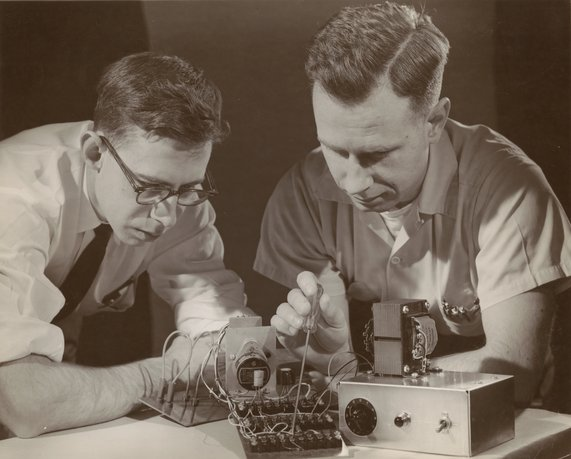
\includegraphics[scale=0.875]{10_deep_learning/02_img/perceptron_rosenblatt}
			\end{figure}
		\end{boxBlueNoFrame}
	}

	\divideTwo{0.49}{
		\begin{boxBlueNoFrame}
			\begin{figure}
				\centering
				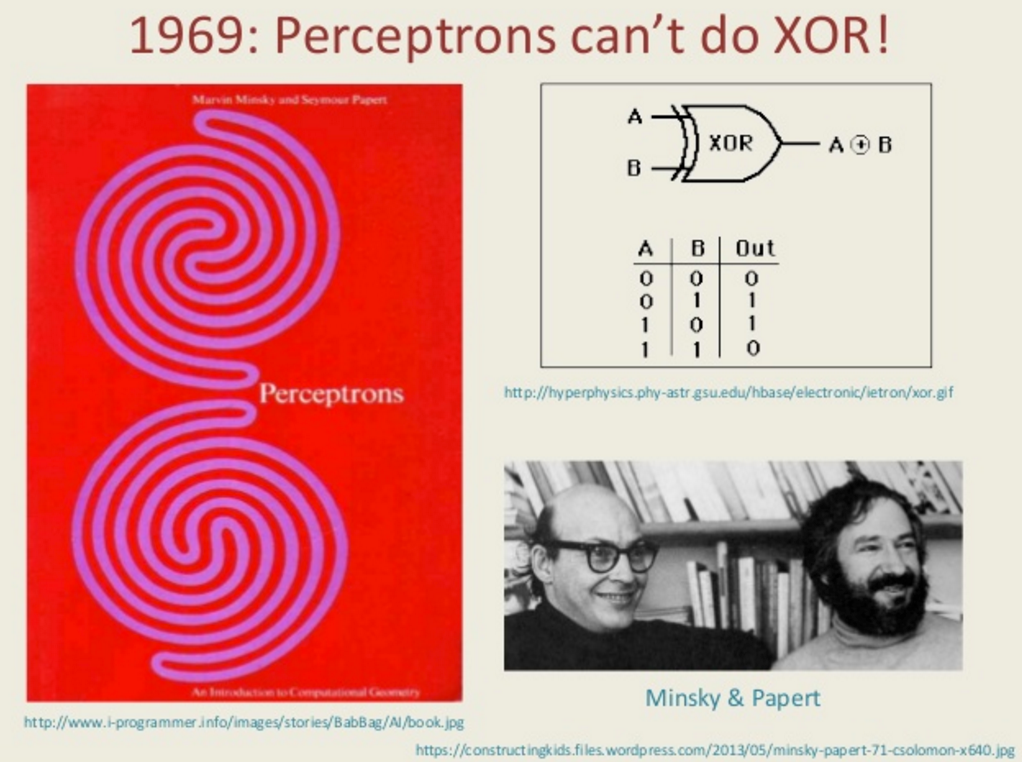
\includegraphics[scale=0.19]{10_deep_learning/02_img/perceptron_xor}
			\end{figure}
		\end{boxBlueNoFrame}
	}{0.49}{
		\begin{boxBlueNoFrame}
			\textbf{Setback I} (mid 1960s -- late 1970s) \\

			\textit{M.\,Minsky} and \textit{S.\,Papert} (1969): \\
			Serious problems with perceptron algorithm:
			It cannot learn the \textbf{XOR problem}.
		\end{boxBlueNoFrame}
	}
\end{frame}


% History of Deep Learning (Ctd.)
\begin{frame}{History of Deep Learning (Ctd.)}{}
	\footnotesize
	\divideTwo{0.49}{
		\begin{boxBlueNoFrame}
			\textbf{Renewed enthusiasm} (1980s)
			\begin{itemize}
				\setlength\itemsep{0.15em}
				\item New techniques available
				\item \highlight{Backpropagation} for deep nets
			\end{itemize}	
		\end{boxBlueNoFrame}

		\begin{boxBlueNoFrame}
			\textbf{Setback II} (1990s -- mid 2000s)
			\begin{itemize}
				\setlength\itemsep{0.15em}
				\item Other techniques were considered superior (e.\,g. SVMs)
				\item CS journals rejected papers on neural networks
			\end{itemize}
		\end{boxBlueNoFrame}
	}{0.49}{
		\begin{boxBlue}
			\textbf{`Deep Learning'} (since mid 2000) \\ \vspace*{1mm}

			More data, faster computers, better optimization techniques...

			\begin{figure}
				\centering
				
\includegraphics[scale=0.275]{10_deep_learning/02_img/deep_learning}
			\end{figure}
		\end{boxBlue}
	}
\end{frame}


% Subsection: Biological Motivation
% --------------------------------------------------------------------------------------------------------
\subsection{Biological Motivation}

% Biological Motivation
\begin{frame}{Biological Motivation}{}
	\begin{itemize}
		\item All neurons are connected and form a complex \textbf{network}
		\item \textbf{Transmitter chemicals} within the fluid of the brain influence the
			\textbf{electrical potential} inside the body of the neurons
		\item If the \textbf{membrane potential} reaches some threshold, the neurons \textbf{fires} \\
			$\Rightarrow$ A pulse of fixed length is sent down the \textbf{axon}
		\item The axon connects the neuron with other neurons (via \textbf{synapses})
		\item Probably there are 100 trillion \textcolor{red}{\textbf{(!!!)}} synapses in the human brain
		\item \textbf{Refractory period} after a neuron has fired
	\end{itemize}
\end{frame}


% Biological Motivation (Ctd.)
\begin{frame}[plain]{}{}
	\begin{figure}
		\centering
		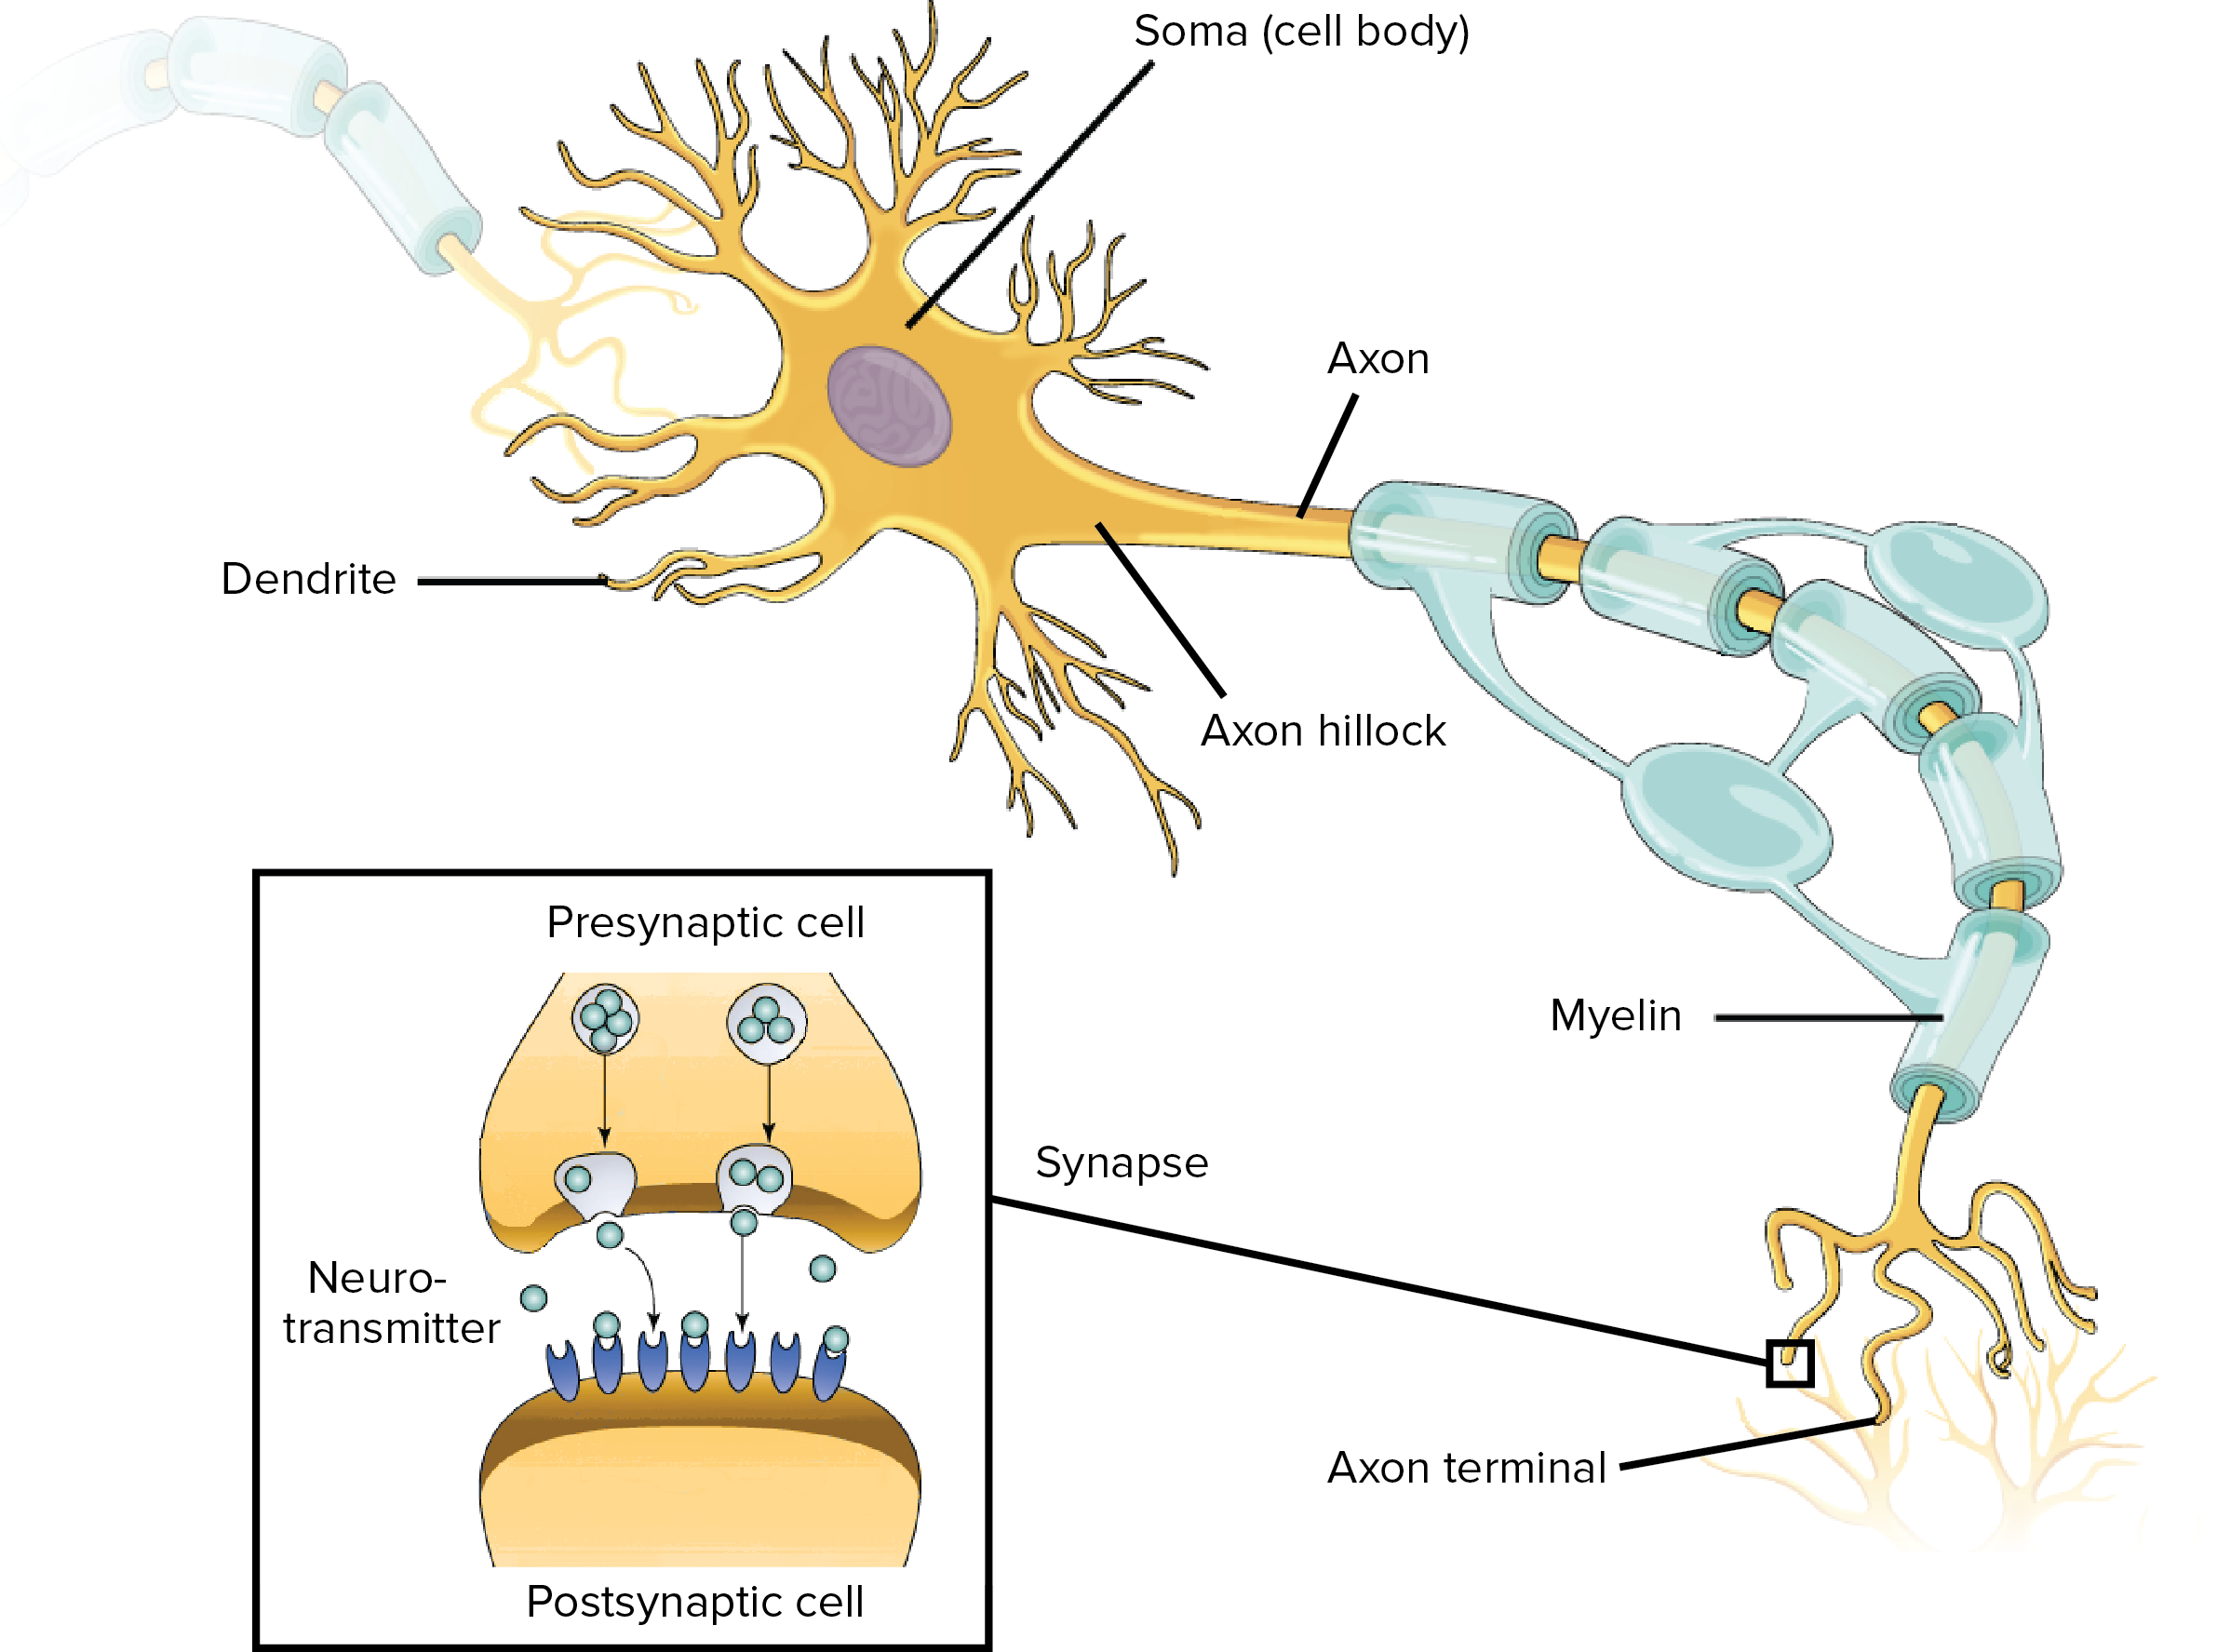
\includegraphics[scale=0.50]{10_deep_learning/02_img/biological_neuron}
	\end{figure}
\end{frame}


% How can we know this?
\begin{frame}{How can we know this?}{}
	\divideTwo{0.29}{
		\begin{figure}
			\centering
			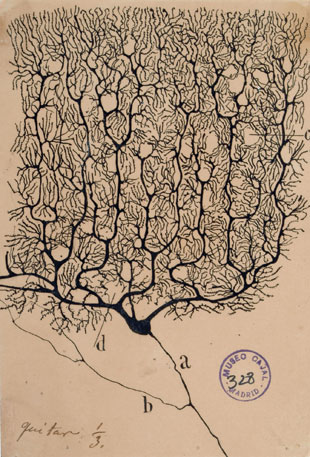
\includegraphics[scale=0.15]{10_deep_learning/02_img/cajal_golgi_stain}
		\end{figure}
	}{0.69}{
		\footnotesize
		\begin{itemize}
			\item \textit{Santiago Ramón y Cajal} made neurons visible by applying \textbf{Golgi's method}
			\item Golgi's method uses the \textbf{Golgi stain} to colorize the neurons
		\end{itemize}
	} \\
	\vspace*{3mm}
	\divideTwo{0.59}{
		\footnotesize
		\begin{itemize}
			\item End of the 1940s, \textit{Hodgkin} and \textit{Huxley} started investigating the electrical properties of
				neurons on the squid's axon
			\item The right-hand-side image was the first \textbf{action potential} ever plotted
		\end{itemize}
	}{0.39}{
		\begin{figure}
			\centering
			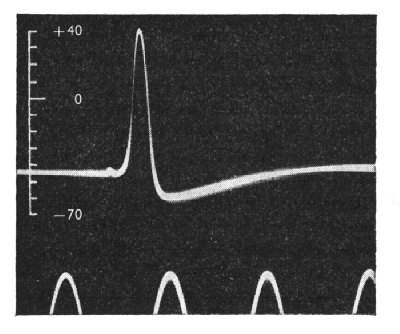
\includegraphics[scale=0.3]{10_deep_learning/02_img/spike_potential_squid}
		\end{figure}
	}
\end{frame}


% How do Humans / Animals learn?
\begin{frame}{How do Humans / Animals learn?}{}
	\footnotesize
	\vspace*{-2mm}
	\begin{itemize}
		\item \textbf{Idea:} Mechanism of learning is \highlight{association}
		\item \highlight{Hebbian learning:} If the firing of one neuron repeatedly assists in firing another neuron,
			the synaptic connection will be strengthened
	\end{itemize}
	
	\begin{boxBlueNoFrame}
		\textit{`When an axon of cell A is near enough to excite a cell B and repeatedly or persistently \textbf{takes part in
			firing it}, some growth process or \textbf{metabolic change} takes place in one or both cells such that
			A's \textbf{efficiency}, as one of the cells firing B, is \textbf{increased}.'} \\[-3mm]

		\textit{`The general idea is an old one, that any two cells or systems of cells that are
			\textbf{repeatedly active at the same} time will tend to become \textbf{`associated'}, so that activity
			in one facilitates activity in the other.'} \hfill \textit{Hebb}
	\end{boxBlueNoFrame}
\end{frame}


% Classical / Pavlovian Conditioning
\begin{frame}{Classical / Pavlovian Conditioning}{}
	\footnotesize
	\divideTwo{0.55}{
		\begin{itemize}
			\item Dog salivates when given food
			\item Food is an \highlight{unconditioned stimulus (US)}
			\item Salivation in response to food is \highlight{unconditioned response (UR)}
			\item Food is paired with the sound of a bell
			\item Bell is  \highlight{conditioned stimulus (CS)}
			\item Bell will eventually elicit salivation event without food
			\item Salivation is  \highlight{conditioned response (CR)}
		\end{itemize}
	}{0.43}{
		\begin{figure}
			\centering
			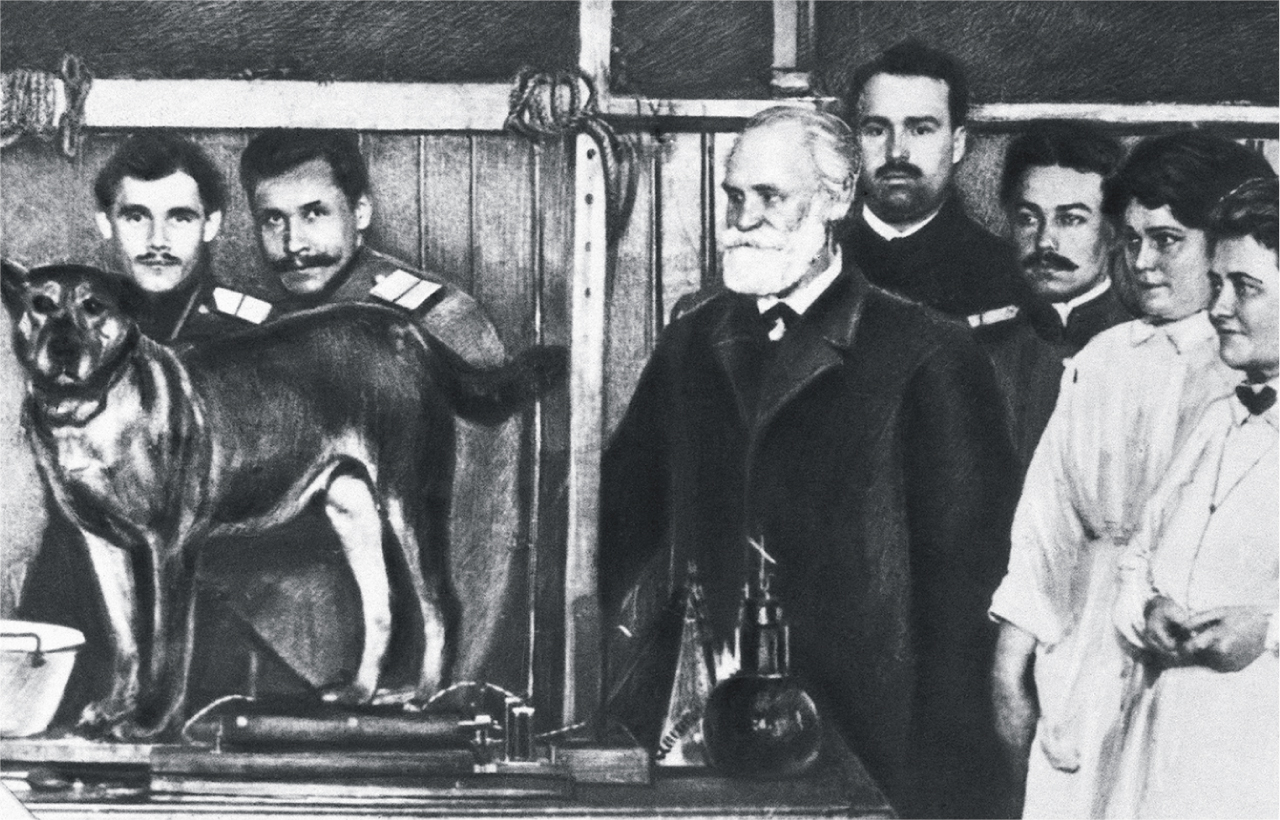
\includegraphics[scale=0.50]{10_deep_learning/02_img/pavlov}
		\end{figure}
	}
\end{frame}


% Classical / Pavlovian Conditioning (Ctd.)
\begin{frame}{Classical / Pavlovian Conditioning (Ctd.)}{}
	\begin{figure}
		\centering
		
\includegraphics[scale=0.70]{10_deep_learning/02_img/pavlov_meme}
	\end{figure}
\end{frame}


% Blocking
\begin{frame}{Blocking}{}
	\begin{table}[h]
	\scalebox{0.75}{
	\begin{tabular}{| l | l | l | l | l |}
		\hline
		\textbf{Group A}	&	train N+	&	train LN+ 	&	test L- 	& 	$\Rightarrow$ no conditioning	\\ \hline
		\textbf{Group B}	&			&	train LN+	&	test L- 	&	$\Rightarrow$ conditioning	\\ \hline
	\end{tabular}}
\end{table}
	
	\footnotesize
	\begin{itemize}
		\item CS is a light (L), a noise (N), or a combination of both (LN)
		\item US is a mild shock that is paired with the CS in the training phase (+)
		\item Fear response is tested after training when only L is presented without shock (-)
		\item Group B shows conditioning; Group A does not: \textbf{N blocks L}
		\item This is hard to explain with Hebbian learning
		\item \textbf{Idea:} Learning only happens, if there is a \highlight{prediction error}
	\end{itemize}
\end{frame}


% Prediction Error -- Dopamine
\begin{frame}[plain]{}{}
	\begin{figure}
		\centering
		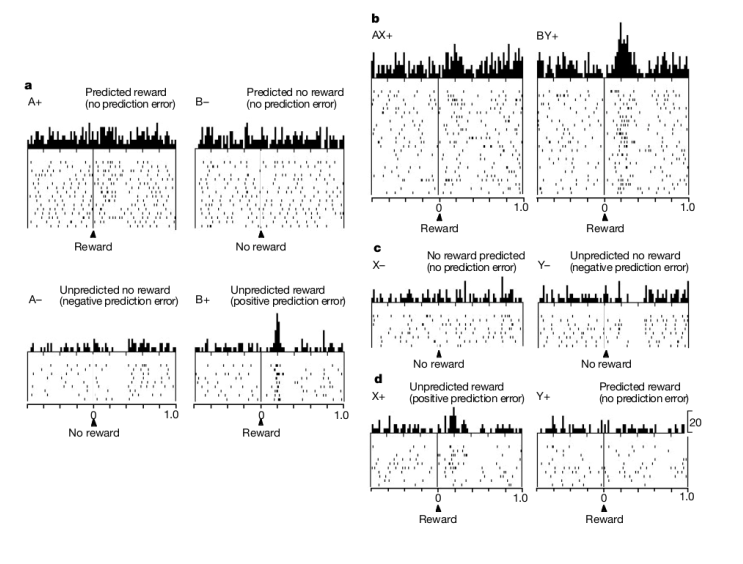
\includegraphics[scale=0.60]{10_deep_learning/02_img/dopamine_prediction_error}
	\end{figure}
\end{frame}


% Artificial Neurons [\textit{McCulloch} and \textit{Pitts}, 1943]
\begin{frame}{Artificial Neurons [\textit{McCulloch} and \textit{Pitts}, 1943]}{}
	\begin{itemize}
		\item In 1943, \textit{McCulloch} and \textit{Pitts} designed the first `artificial neuron'
		\item These neurons can represent logical functions (e.\,g. b: \texttt{OR}, c: \texttt{AND})
	\end{itemize}
	
	\begin{figure}
		\centering
		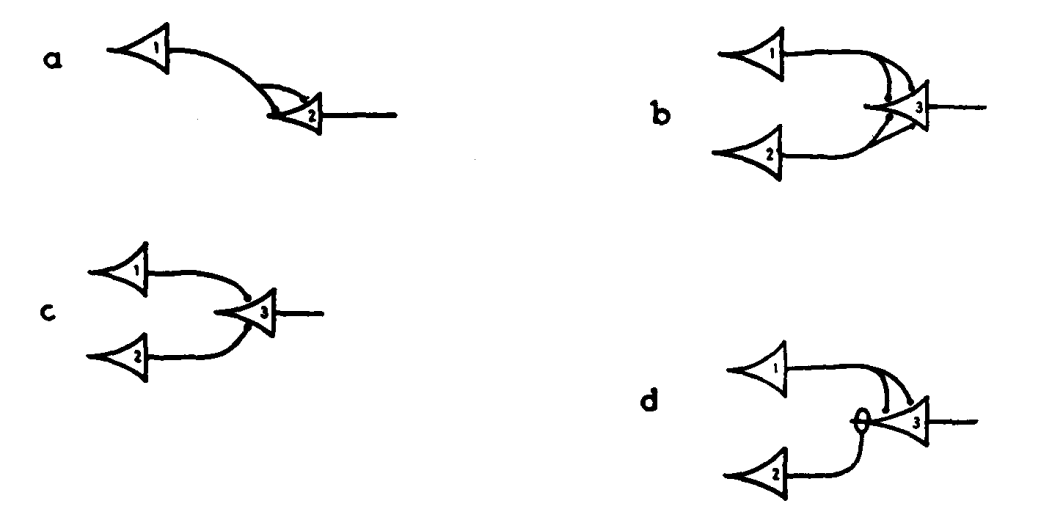
\includegraphics[scale=0.25]{10_deep_learning/02_img/mcculloch_pitts}
	\end{figure}
\end{frame}


% Section: Perceptrons
%______________________________________________________________________
\section{Perceptrons}
\makedivider{Perceptrons}

% Subsection: The original Perceptron Algorithm
% --------------------------------------------------------------------------------------------------------
\subsection{The original Perceptron Algorithm}

% Original Perceptron Algorithm [\textit{Rosenblatt}, 1957]
\begin{frame}{Original Perceptron Algorithm [\textit{Rosenblatt}, 1957]}{}
	\begin{enumerate}
		\item Initialize the weight vector $\bm{\theta}$ and a bias $b$
		\item $\forall (\bm{x}_i \in \bm{X}, y_i \in \{ -1, +1 \})_{i=1}^n$ (until convergence):
		\begin{itemize}
			\item[\textbf{2a)}] If $\bm{x}_i$ is correctly classified, do nothing
			\item[\textbf{2b)}] Else if $y_i = +1$, update the paramters with:
			\begin{equation*}
				\bm{w} \longleftarrow \bm{w} + \bm{x}_i \qquad\qquad b \longleftarrow b + 1
			\end{equation*}
			\item[\textbf{2c)}] Else if $y_i = -1$, update the paramters with:
			\begin{equation*}
				\bm{w} \longleftarrow \bm{w} - \bm{x}_i \qquad\qquad b \longleftarrow b - 1
			\end{equation*}
		\end{itemize}
	\end{enumerate}
\end{frame}


% Original Perceptron Algorithm (Ctd.)
\begin{frame}{Original Perceptron Algorithm (Ctd.)}{}
	\begin{figure}
		\centering
		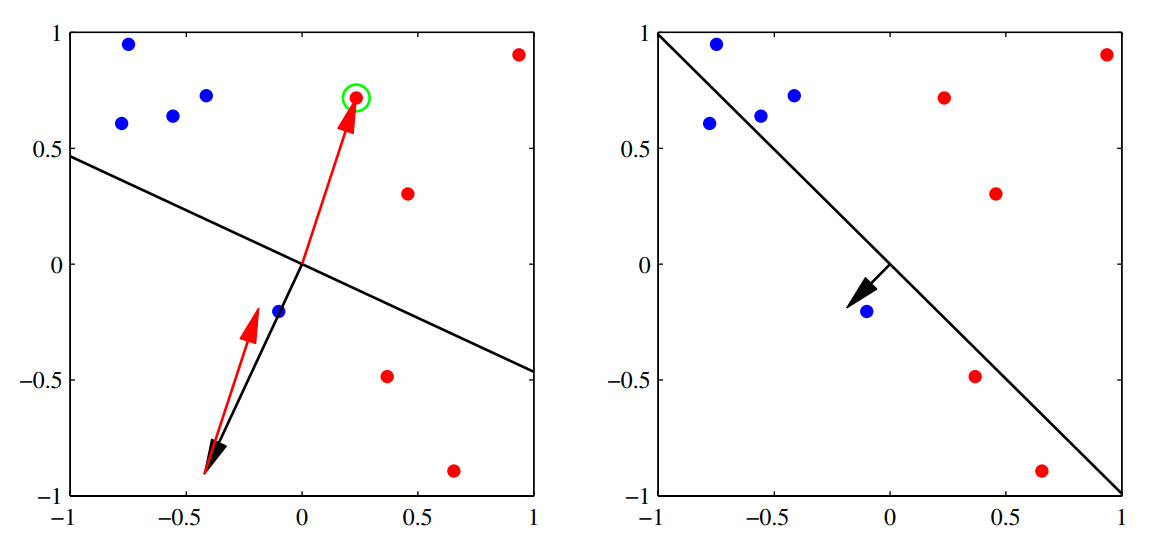
\includegraphics[scale=0.35]{10_deep_learning/02_img/perceptron_1}
	\end{figure}
	\citeAuthor{cf.}{Bishop.2006}{p. 195}
\end{frame}


% Original Perceptron Algorithm (Ctd.)
\begin{frame}{Original Perceptron Algorithm (Ctd.)}{}
	\begin{figure}
		\centering
		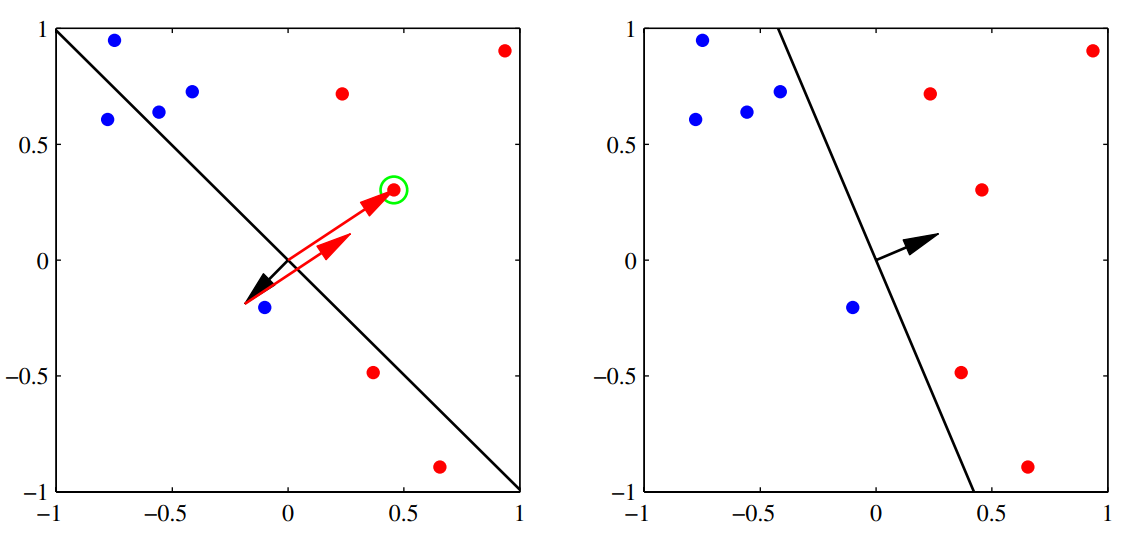
\includegraphics[scale=0.35]{10_deep_learning/02_img/perceptron_2}
	\end{figure}
	\citeAuthor{cf.}{Bishop.2006}{p. 195}
\end{frame}


% Perceptron Convergence Theorem
\begin{frame}{Perceptron Convergence Theorem}{}
	\begin{boxBlue}
		\highlight{Perceptron Convergence Theorem} \\

		If the training data is \textbf{linearly separable}, then the perceptron learning algorithm is going to
		\textbf{converge after a finite amount of time} and classifies \textbf{all training data examples correctly}.
	\end{boxBlue}
\end{frame}


% Subsection: `New' Perceptron Learning Algorithm
% --------------------------------------------------------------------------------------------------------
\subsection{`New' Perceptron Learning Algorithm}

% The Architecture of a Neuron
\begin{frame}{The Architecture of a Neuron}{}
	\begin{figure}
	\centering
	\begin{tikzpicture}[
		scale=0.8
	]

		\node[circle,draw=black,minimum size=4cm,thick] (N) at (0,0) {};

		\foreach \y/\i in {1.5/1,0/2,-1.5/3,-3/4}{
			\draw[thick] (-8,\y) -- node[above] {$\theta_{\i}$} (N);
			\node[circle,draw=black,fill=white,thick] at (-8,\y) {$x_{\i}$};
		}

		\draw[thick] (-8,3) -- node[above] {$\theta_{0}$} (N);
		\node[circle,thick,draw=black,fill=black,thick] at (-8,3) {\textcolor{white}{\textbf{1}}};

		\draw[thick] (N) -- ++(6,0) node[right] {z};

		\draw[pattern=north west lines,pattern color=purple!30] (0,2.4) arc (90:270:2.4) -- cycle;
		\draw[pattern=north west lines,pattern color=orange!30] (0,2.4) arc (90:-90:2.4) -- cycle;
		\node at (-1.25,0) {$a = \bm{\theta}^{\intercal} \bm{x}$};
		\node at (1.25,0) {$z = \sigma(a)$};

		\node[purple,align=center] at (-1.15,1) {\scriptsize \textbf{pre-}\\[-2mm] \scriptsize \textbf{activation}};
		\node[orange] at (1.15,1) {\scriptsize \textbf{activation}};
		\node[rotate=90,gray] at (-9,0) {\footnotesize \textbf{input}};
		\node[rotate=90,gray] at (7,0) {\footnotesize \textbf{output}};

	\end{tikzpicture}
\end{figure}
\end{frame}


% Perceptron
\begin{frame}{Perceptron}{}
	\begin{itemize}
		\item The neuron receives an input vector $\bm{x}$:
		\begin{equation*}
			\bm{x} = (1, x_1, x_2, \dots, x_m)^{\intercal}
		\end{equation*}
		\item Each input signal is weighted by a factor $\theta_j$: {\footnotesize\textit{(weight of synaptic strength)}}
		\begin{equation*}
			\bm{\theta} = (\theta_0, \theta_1, \theta_2, \dots, \theta_m)^{\intercal}
		\end{equation*}
		\item We compute the \highlight{pre-activation} and the \highlight{activation}:
		\begin{equation}
			a = \bm{\theta}^{\intercal} \bm{x} = \sum_{j=0}^m \theta_j x_j \qquad\qquad
			z = \sigma(a)
		\end{equation}
	\end{itemize}
\end{frame}


% Perceptron (Ctd.)
\begin{frame}{Perceptron (Ctd.)}{}
	\begin{itemize}
		\item The simplest activation function is to use a threshold\footnote[frame]{Not used, since not differentiable;
			alternatives later} $\rho$:
		\begin{equation*}
			\sigma_{\rho}(a) =
			\begin{cases}
				0 &	\text{for}\ a \le \rho \\
				1 & \text{for}\ a > \rho
			\end{cases}
		\end{equation*}
		\item Quick example: $\bm{x} = (1, 0, 0.5)^{\intercal} \qquad \bm{\theta} = (1, -0.5, -1)^{\intercal} \qquad \rho = 0$
		\begin{align*}
			a &= \bm{\theta}^{\intercal}\bm{x} = 1 \cdot 1 + (-0.5) \cdot 0 + (-1) \cdot 0.5 = 0.5 \\
			z &= \sigma_{\rho=0}(0.5) = 1
		\end{align*}
	\end{itemize}
\end{frame}


% Perceptron Learning
\begin{frame}{Perceptron Learning}{}
	\begin{itemize}
		\item Learning means choosing the correct weights $\bm{\theta}^*$ from a set of possible hypotheses $\mathcal{H}$
		(\highlight{hypothesis space}):
		\begin{equation*}
			\mathcal{H} = \{ \bm{\theta} \vert \bm{\theta} \in \mathbb{R}^{m + 1} \}
		\end{equation*}
		\item How to learn the weights from a data set $\mathcal{D}$?
		\item \textbf{Algorithm outline:}
		\begin{enumerate}
			\item Pick a training example $\bm{x} \in \mathcal{D}$
			\item Calculate the activation $z$ for that training example
			\item Update the weights $\bm{\theta}$ based on the error
		\end{enumerate}
	\end{itemize}
\end{frame}


% Perceptron Learning (Ctd.)
\begin{frame}{Perceptron Learning (Ctd.)}{}
	\begin{itemize}
		\item How can we compute the error? $\Rightarrow$ We need a loss function $\mathcal{J}(\bm{\theta})$:
		\begin{equation}
			\mathcal{J}(\bm{\theta}) = \frac{1}{2} \sum_{i=1}^n (h_{\bm{\theta}}(\bm{x}^{(i)}) - y^{(i)})^2
		\end{equation}
		\item Again, we use \highlight{gradient descent}: Compute gradient and go into the negative direction of the gradient:
		\begin{equation}
			\bm{\theta}^{(t+1)} \longleftarrow \bm{\theta}^{(t)} - \alpha \nabla_{\bm{\theta}} \mathcal{J}(\bm{\theta})
		\end{equation}
	\end{itemize}
	\textcolor{gray}{$\Rightarrow$ cf. slides `Regression'}
\end{frame}


% Generalization to multiple Classes
\begin{frame}{Generalization to multiple Classes}{}
	\divideTwo{0.59}{
		\footnotesize
		\begin{itemize}
			\item A single neuron can only distinguish two classes
			\item If there are more than two classes: Simply use more neurons\footnote[frame] {This construct is still
				referred to as a perceptron.}
			\item Use \highlight{one-hot encoding} for the classes and \highlight{softmax} as activation function (later)
			\item Example for three classes:
			\begin{tabbing}
				\hspace*{1cm}\=\kill
				$\mathcal{C}_1$ \> \texttt{1 0 0} \\
				$\mathcal{C}_2$ \> \texttt{0 1 0} \\
				$\mathcal{C}_3$ \> \texttt{0 0 1}
			\end{tabbing}
		\end{itemize}	
	}{0.39}{
		\begin{figure}
	\centering
	\begin{tikzpicture}[
		scale=0.6,
		every node/.style={scale=0.8}
	]

		\foreach \y in {-3,-1.5,0,1.5,3}{
			\foreach \yy in {-2,0,2}{
				\draw (-5,\y) -- (0,\yy);
			}
		}
	
		% input layer
		\foreach \y/\i in {3/1,1.5/2,0/3,-1.5/4,-3/5}{
			\node[circle,draw=black,fill=lightgray] at (-5,\y) {$x_{\i}$};
		}
		
		% rbf layer
		\foreach \y/\i in {-2/3,0/2,2/1}{
			\node[circle,draw=black,fill=white,align=center] at (0,\y) {$P_{\i}$};
		}
		\node at (1.5,2) {\texttt{0}};
		\node at (1.5,0) {\texttt{1}};
		\node at (1.5,-2) {\texttt{0}};

		\node[rotate=90,gray] at (-6.5,0) {\footnotesize \textbf{input}};
		\node[rotate=90,gray] at (2.5,0) {\footnotesize \textbf{output}};

	\end{tikzpicture}
\end{figure}
	}
\end{frame}


% What about non-linear Data Sets?
\begin{frame}{What about non-linear Data Sets?}{}
	\divideTwo{0.39}{
		\begin{itemize}
			\item Perceptrons cannot learn non-linear boundaries
			\item Remember \textit{Minsky} and \textit{Papert}
			\item What can we do?
			\begin{enumerate}
				\item Add feature mapping {\scriptsize(cf. right)}
				\item Add hidden layers \\
					{\scriptsize\highlight{(Multi-Layer Perceptrons)}}
			\end{enumerate}
	\end{itemize}
	}{0.59}{
		\begin{figure}
			\centering
			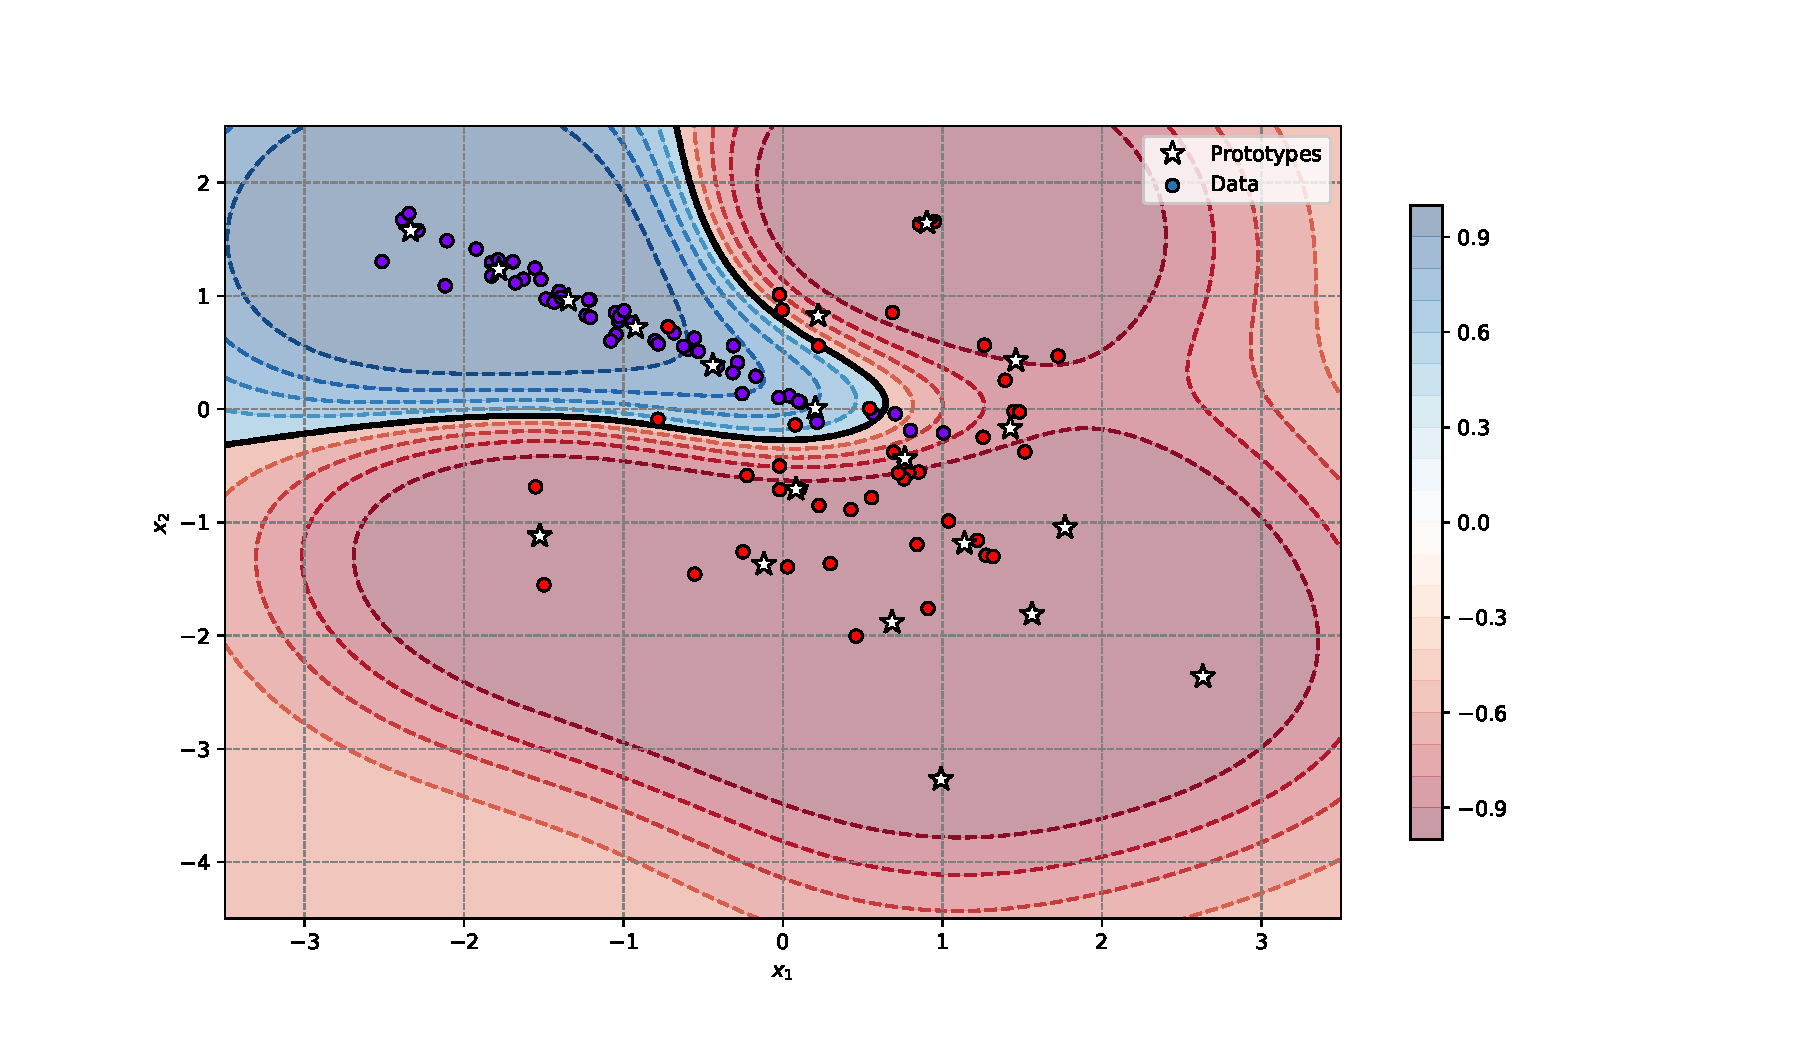
\includegraphics[scale=0.35]{10_deep_learning/02_img/rbfn}
		\end{figure}
	}
\end{frame}


% Section: Multi-Layer-Perceptrons (MLPs)
%______________________________________________________________________
\section{Multi-Layer-Perceptrons (MLPs)}
\makedivider{Multi-Layer-Perceptrons (MLPs)}


% Subsection: MLP
% --------------------------------------------------------------------------------------------------------
\subsection{Overview}

% Multi-Layer Perceptrons
\begin{frame}{Multi-Layer Perceptrons}{}
	\begin{itemize}
		\item In theory, a \highlight{Multi-Layer Perceptron (MLP)} can approximate any continuous function arbitrarily well
		\item An MLP with $\lambda$ hidden layers is a function $h: \mathbb{R}^m \rightarrow \mathbb{R}^{\kappa}$,
			parameterized by network parameters $\bm{\Theta}^{(1)}$, $\bm{\Theta}^{(2)}$, \dots, $\bm{\Theta}^{(\lambda)}$
		\item In each layer, a non-linearity is applied: $g^{(1)}$, $g^{(2)}$, \dots, $g^{(\lambda)}$
	\end{itemize}
	\divideTwo{0.49}{
		\begin{align*}
			z^{(1)} &= g^{(1)}(\bm{\Theta}^{(1)} \bm{x})								\\
			\dots 													\\
			z^{(\lambda)} &= \bm{\Theta}^{(\lambda)} g^{(\lambda - 1)}(\bm{z}^{(\lambda - 1)})
		\end{align*}
	}{0.49}{
		\begin{align*}
			\bm{h} &= g^{(\lambda)}(\bm{z^{(\lambda)}}) 						\\
			y_{pred} &= \argmax_k \bm{h}
		\end{align*}
	}
\end{frame}


% MLP Learning
\begin{frame}{MLP Learning}{}
	\begin{enumerate}
		\item Start by randomly initializing the network weights
		\item \Highlight{Do not set an initial value of 0 for all weights! (Why?)} \\
			$\Rightarrow$ Initialize to small random numbers
		\item Perform a forward pass through the network, i.\,e. make predictions
		\item Using the predictions, compute a scalar loss value $\mathcal{J}(\bm{\Theta})$
		\item Calculate the gradients of the loss w.\,r.\,t. each network parameter and update all parameters (gradient descent)
	\end{enumerate}
\end{frame}


% Subsection: Backpropagation
% --------------------------------------------------------------------------------------------------------
\subsection{Backpropagation}

% Backpropagation
\begin{frame}{Backpropagation}{}\important
	\begin{itemize}
		\item In order to update the weights, we first have to perform a \highlight{forward pass}:
		\begin{align*}
			h_k(\bm{x}^{(i)}; \bm{\Theta})
				&= g^{(2)}\left( \sum_{l=0}^h \Theta_{kl}^{(2)} g^{(1)}\left( \sum_{j=0}^m \Theta_{lj}^{(1)} x_{j}^{(i)} \right) \right) \\
			z_l
				&=  g^{(1)}\left( \sum_{j=0}^m \Theta_{lj}^{(1)} x_{j}^{(i)} \right) \qquad\text{activation}
		\end{align*}
		\item $g(\cdot) \equiv$ activation function, e.\,g. sigmoid, tanh, ReLU
		\item $\bm{\Theta}$ are the network parameters (to be learned)
	\end{itemize}
\end{frame}


% Backpropagation (Ctd.)
\begin{frame}[plain]{}{}
	\bubble{0.5}{0.5}{
		\tiny This is a fully connected \\[-2mm]
		\tiny neural network
	}
	\begin{figure}
	\centering
	\begin{tikzpicture}[
		scale=0.8,
		b/.style={circle,fill=black,minimum width=7mm},
		n/.style={circle,draw=black,fill=white,very thick,minimum width=7mm}
	]
		
		\foreach \y in {3,6}{
			\foreach \i in {-4.5,-1.5,1.5,7.5}{
				\foreach \j in {-1.5,1.5,7.5}{
					\draw (\i, \y-3) -- (\j,\y);
				}
			}
		}
		
		% input layer
		\node[b] at (-4.5,0) {\footnotesize\textcolor{white}{\textbf{1}}};
		\node[n] at (-1.5,0) {};
		\node[n] at (1.5,0) {};
		\node at (4.5,0) {$\dots$};
		\node[n] at (7.5,0) {};

		% hidden layer
		\node[b] at (-4.5,3) {\footnotesize\textcolor{white}{\textbf{1}}};
		\node[n] at (-1.5,3) {};
		\node[n] at (1.5,3) {};
		\node at (4.5,3) {$\dots$};
		\node[n] at (7.5,3) {};

		% output layer
		\node[n] at (-1.5,6) {};
		\node[n] at (1.5,6) {};
		\node at (4.5,6) {$\dots$};
		\node[n] at (7.5,6) {};

		% input
		\node at (-4.5,-1) {$x_0$};
		\node at (-1.5,-1) {$x_1$};
		\node at (1.5,-1) {$x_2$};
		\node at (4.5,-1) {$\dots$};
		\node at (7.5,-1) {$x_m$};
		
		% output
		\node at (-1.5,7) {$h_1$};
		\node at (1.5,7) {$h_2$};
		\node at (4.5,7) {$\dots$};
		\node at (7.5,7) {$h_{\kappa}$};

		% hidden
		\node at (-5.5,3) {$z_0$};
		\node at (-2.5,3) {$z_1$};
		\node at (8.5,3) {$z_h$};

		% weights
		\node at (-4,1.5) {$\bm{\Theta}^{(1)}$};
		\node at (-4,4.5) {$\bm{\Theta}^{(2)}$};
		
		\node at (10,0) {\highlight{input}};
		\node at (10,3) {\highlight{hidden}};
		\node at (10,6) {\highlight{output}};
		
	\end{tikzpicture}
\end{figure}
\end{frame}


% Backpropagation (Ctd.)
\begin{frame}{Backpropagation (Ctd.)}{}\important
	\begin{itemize}
		\item Compute the network loss
		\item The loss function is given by: {\footnotesize(assume square loss: $\ell = (h_k(\bm{x}^{(i)}; \bm{\Theta}) - y_k^{(i)})^2$)}
		\begin{equation*}
			\mathcal{J}(\bm{\Theta}) = \frac{1}{n} \sum_{i=1}^n \sum_{k=1}^\kappa
				\ell(h_k(\bm{x}^{(i)}; \bm{\Theta}), y_k^{(i)})
		\end{equation*}
		\item Compute the error gradient w.\,r.\,t. $h_k(\bm{x}^{(i)}; \bm{\Theta})$:
		\begin{equation*}
			 \frac{\partial \mathcal{J}^{(i)}(\bm{\Theta})}{\partial h_k(\bm{x}^{(i)}; \bm{\Theta})}
			 	= \ell'(h_k(\bm{x}^{(i)}; \bm{\Theta}), y_k^{(i)}) \equiv \delta_k^{(i)}
		\end{equation*}
	\end{itemize}
\end{frame}


% Backpropagation (Ctd.)
\begin{frame}{Backpropagation (Ctd.)}{}\important
	\begin{itemize}
		\item Compute the weight gradient for the output layer:
		\begin{align*}
			\frac{\partial \mathcal{J}^{(i)}(\bm{\Theta})}{\partial \Theta_{kl}^{(2)}}
				&= \frac{\partial \mathcal{J}(\bm{\Theta})}{\partial h_k(\bm{x}^{(i)}; \bm{\Theta})}
					\frac{\partial h_k(\bm{x}^{(i)}; \bm{\Theta})}{\partial \Theta_{kl}^{(2)}} \\
				&= \ell'(h_k(\bm{x}^{(i)}; \bm{\Theta}), y_k^{(i)}) \cdot g'^{(2)} \left( \sum_{t=0}^h \Theta_{kt}^{(2)} z_t(\bm{x}^{(i)}) \right)
					\cdot z_l(\bm{x}^{(i)}) \\
				&= \delta_k^{(i)} \cdot g'^{(2)} \left( \sum_{t=0}^h \Theta_{kt}^{(2)} z_t(\bm{x}^{(i)}) \right) \cdot z_l(\bm{x}^{(i)})
		\end{align*}
	\end{itemize}
\end{frame}


% Backpropagation (Ctd.)
\begin{frame}{Backpropagation (Ctd.)}{}\important
	\begin{itemize}
		\item Compute the error gradient for the hidden layer:
		\begin{align*}
			\frac{\partial \mathcal{J}^{(i)}(\bm{\Theta})}{\partial z_l}
				&= \sum_{k=1}^\kappa \frac{\partial \mathcal{J}^{(i)}(\bm{\Theta})}{\partial h_k(\bm{x}^{(i)}; \bm{\Theta})}
					\frac{\partial h_k(\bm{x}^{(i)}; \bm{\Theta})}{\partial z_l} \\
				&= \sum_{k=1}^\kappa \ell'(h_k(\bm{x}^{(i)}; \bm{\Theta}), y^{(i)})
					\cdot g'^{(2)}\left( \sum_{t=0}^h \Theta_{kt}^{(2)} z_t(\bm{x}^{(i)}) \right) \cdot \Theta_{kl}^{(2)} \\
				&= \sum_{k=1}^\kappa \delta_k^{(i)} \cdot g'^{(2)} \left( \sum_{t=0}^h \Theta_{kt}^{(2)} z_t(\bm{x}^{(i)}) \right)
					\cdot \Theta_{kl}^{(2)} \equiv \widehat{\delta}_l^{(i)}
		\end{align*}
	\end{itemize}
\end{frame}


% Backpropagation (Ctd.)
\begin{frame}{Backpropagation (Ctd.)}{}\important
	\begin{itemize}
		\item Compute the weight gradient for the hidden layer:
		\begin{align*}
			\frac{\partial \mathcal{J}^{(i)}(\bm{\Theta})}{\partial \Theta_{lj}^{(1)}}
				&= \frac{\partial \mathcal{J}^{(i)}(\bm{\Theta})}{\partial z_l} \cdot g'^{(1)} \left( \sum_{t=0}^m \Theta_{lt}^{(1)} x_t^{(i)} \right) \cdot x_j^{(i)} \\
				&= \widehat{\delta}_l^{(i)} \cdot g'^{(1)} \left( \sum_{t=0}^m \Theta_{lt}^{(1)} x_t^{(i)} \right) \cdot x_j^{(i)}
		\end{align*}
		\item The weight derivatives are now used in the gradient descent update rule
	\end{itemize}
\end{frame}


% Backpropagation Example
\begin{frame}{Backpropagation Example}{}
	\vfill
	\begin{center}
		\Huge \highlight{See blackboard!}
	\end{center}
	\vfill
\end{frame}


% Some Remarks
\begin{frame}{Some Remarks}{}
	\begin{itemize}
		\item \textbf{Check your gradients:}
		\begin{equation*}
			\nabla h(x) \overset{!}{\approx} \frac{1}{\varepsilon} \cdot (h(x + \varepsilon) - h(x))
		\end{equation*}
		\item \textbf{Hyper-parameter optimization is necessary:}
	\end{itemize}
	\divideTwo{0.49}{
		\footnotesize
		\begin{itemize}\setlength\itemsep{-0.5em}
			\item \# hidden layers
			\item \# hidden units
			\item activation functions
			\item learning rate
		\end{itemize}
	}{0.49}{
		\footnotesize
		\begin{itemize}\setlength\itemsep{-0.5em}
			\item batch size
			\item \# training epochs
			\item regularization
			\item ...	
		\end{itemize}
	}
	\begin{itemize}
		\item Have a look at: \url{https://playground.tensorflow.org}
	\end{itemize}
\end{frame}


% Subsection: Backpropagation
% --------------------------------------------------------------------------------------------------------
\subsection{Activation Functions}

% Sigmoid Function
\begin{frame}{Sigmoid Function}{}
	\begin{boxBlueNoFrame}
		\begin{equation*}
			\sigma(x) = \frac{1}{1 + e^{-x}} \qquad\qquad
			\sigma'(x) = \sigma(x) (1 - \sigma(x))
		\end{equation*}
	\end{boxBlueNoFrame}

	\begin{itemize}
		\item Value range: 0 to 1
		\item \Highlight{Problem 1:} Gradient can become very small \textbf{(vanishing gradient problem)}
		\item \Highlight{Problem 2:} Output is not zero-centered (makes optimization harder)
	\end{itemize}
\end{frame}


% Sigmoid Function (Ctd.)
\begin{frame}{Sigmoid Function (Ctd.)}{}
	\begin{boxBlueNoFrame}
		\footnotesize
		\textit{`Convergence is usually faster if the average of each input variable over the training set is close to zero.
		To see this, consider the extreme case where all the inputs are positive. Weights to a particular node in the first weight layer are updated by an amount
		proportional to $\delta$x where $\delta$ is the (scalar) error at that node and x is the input vector. When all of the components of an input vector are
		positive, all of the updates of weights that feed into a node will have the same sign (i.\,e. sign($\delta$)). As a result, these weights can only all decrease
		or all increase together for a given input pattern. Thus, if a weight vector must change direction it can only do so by zigzagging which is inefficient and thus
		very slow.'} - \textbf{Yann LeCun et al., Efficient BackProp, 1998} (\url{http://yann.lecun.com/exdb/publis/pdf/lecun-98b.pdf})
	\end{boxBlueNoFrame}
\end{frame}


% Tangent Hyperbolic (tanh)
\begin{frame}{Tangent Hyperbolic (tanh)}{}
	\begin{boxBlueNoFrame}
		\begin{equation*}
			\tanh(x) = \frac{e^x - e^{-x}}{e^x + e^{-x}} \qquad\qquad
			\tanh'(x) = 1 - \tanh(x)^2
		\end{equation*}
	\end{boxBlueNoFrame}
	
	\begin{itemize}
		\item Value range: -1 to 1
		\item Zero-centered
		\item \Highlight{Still suffers from the vanishing gradient problem}
	\end{itemize}
\end{frame}


% Rectified Linear Unit (ReLU)
\begin{frame}{Rectified Linear Unit (ReLU)}{}\important
	\divideTwo{0.49}{
		\begin{itemize}
			\item $ReLU(x) = max(0,x)$
			\item $ReLU'(x) = 
			\begin{cases}
				0 & \text{if}\ x \le 0 \\
				1 & \text{otherwise}
			\end{cases}$
		\end{itemize}
	}{0.49}{
		\begin{figure}
			\centering
			\begin{tikzpicture}[scale=0.6]
				\begin{axis}[domain=-3:5]
					\addplot+[mark=none,red,domain=-3:0,ultra thick] {0};
					\addplot+[mark=none,red,domain=0:5,ultra thick] {x};
				\end{axis}
			\end{tikzpicture}
		\end{figure}
	}
\end{frame}


% ReLU (Ctd.)
\begin{frame}{ReLU (Ctd.)}{}\important
	\begin{itemize}
		\item ReLU does not lead to vanishing gradients
		\item ReLU is very efficient to compute
		\item Use ReLU as the hidden layer activation function!
		\item But: Pay attention to the initialization of your parameters to avoid \textit{`dying ReLUs'} (parameter settings where single neurons will always output 0)
		\item \highlight{Use batch-normalization!}
	\end{itemize}
\end{frame}


% Softmax Activation
\begin{frame}{Softmax Activation}{}
	\begin{boxBlueNoFrame}
		\begin{equation*}
			softmax_k(\bm{x}) = \frac{\exp\{ x_k\}}{\sum_{j=1}^{\kappa} \exp\{x_j\}}
		\end{equation*}
	\end{boxBlueNoFrame}
	\begin{itemize}
		\item Softmax is a \textbf{global activation function} (i.\,e. it depends on the preactivations of the other units in the layer)
		\item It is used to squash the last layer's activations into a probability distribution, \textbf{such that the activations sum to 1}
	\end{itemize}
\end{frame}


% Section: Further Network Architectures and Word Embeddings
%______________________________________________________________________
\section[Further Network Architectures and Word Embeddings]{Further Arch. / Word Emb.}
\makedivider{Further Network Architectures and Word Embeddings}

% Subsection: Convolutional Neural Networks
% --------------------------------------------------------------------------------------------------------
\subsection{Convolutional Neural Networks}

% Convolutional Neural Networks (CNNs)
\begin{frame}{Convolutional Neural Networks (CNNs)}{}
	\begin{itemize}
		\item A fully-connected MLP network has a lot of parameters, i.\,e. it might be \textbf{too complex} or \textbf{computationally inefficient} for some tasks
		\item The input position does not matter in all cases (e.\,g. word positions when classifying emails)
		\item An MLP always needs a fixed-size input vector, but \textbf{we might have variable-size input data}
			(e.\,g. images in different resolutions, text sequences of different lengths, etc.)
		\item \highlight{Solution:} Use \highlight{convolution}!
	\end{itemize}
\end{frame}


% CNN: General Idea
\begin{frame}{CNN: General Idea}{}
	\begin{boxBlueNoFrame}
		\footnotesize
		\textit{`A convolutional neural network is designed to identify indicative local predictors in a large structure, and combine them to produce a fixed size vector
		representation of the structure, capturing these local aspects that are most informative for the prediction task at hand.'} - \textbf{Yoav Goldberg}
	\end{boxBlueNoFrame}
	\begin{itemize}
		\item A CNN consists of multiple convolutional layers
		\item A convolutional layer consists of a filter and a non-linear activation function
		\item \highlight{Pooling} extracts the most important features \textbf{independent of their input position}
	\end{itemize}
\end{frame}


% Convolution
\begin{frame}{Convolution}{}\important
	\begin{boxBlueNoFrame}
		\begin{equation*}
			(x \star g)[i] = \sum_{j=-w}^w x[i - j] \cdot g[j]
		\end{equation*}
	\end{boxBlueNoFrame}
		
	\begin{itemize}
		\item $\star$ is the convolution operator
		\item $x$ is the input to the convolutional layer
		\item $i$ is the current position in the input
		\item $j$ is the filter size / window size
		\item $g$ is the convolution filter (kernel)
	\end{itemize}
\end{frame}


% Convolution (Ctd.)
\begin{frame}{Convolution (Ctd.)}{}\important
	\begin{itemize}
		\item The convolution operation
		\begin{equation*}
			(x \star g)[i] = \sum_{j=-w}^w x[i - j] \cdot g[j]
		\end{equation*}
		\item We shift a filter across the input data (e.\,g. image pixels) with a certain stride and multiply the input with the filter weights at each position
	\end{itemize}
	
	\begin{figure}
		\centering
		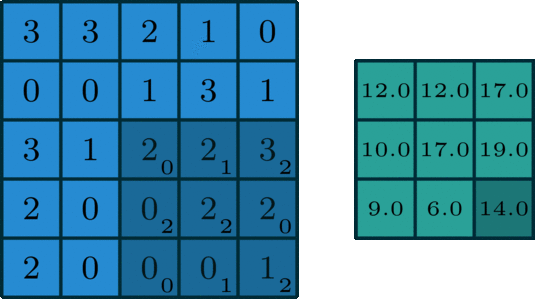
\includegraphics[scale=0.80]{10_deep_learning/02_img/flatconvolution}
	\end{figure}
\end{frame}


% Convolution Animation
\begin{frame}{Convolution Animation}{}\important
	\begin{figure}
		\centering
		\animategraphics[autoplay,loop,height=5.5cm]{2.5}
			{10_deep_learning/02_img/convolution_animation/}{0}{45}
	\end{figure}
\end{frame}


% Pooling
\begin{frame}{Pooling}{}
	\begin{itemize}
		\item The outputs of the convolutions are passed through non-linear activation functions (e.\,g. ReLU, tanh, ...)
		\item Pooling is applied to extract only the most important activations:
		\begin{itemize}
			\item \highlight{max-pooling} (extracts the maximum activation)
			\item \highlight{mean-pooling} (extracts the mean activation)
			\item etc.
		\end{itemize}
		\item \textbf{There are no parameters involved in the pooling operation}
		\item In image processing, pooling is necessary to reduce the dimensionality
	\end{itemize}
\end{frame}


% Subsection: Recurrent Neural Networks
% --------------------------------------------------------------------------------------------------------
\subsection{Recurrent Neural Networks}

% Recurrent Neural Networks
\begin{frame}{Recurrent Neural Networks (RNNs)}{}
	\begin{itemize}
		\item \highlight{Recurrent Neural Networks (RNNs)} can be used to process sequences
		\begin{itemize}
			\item Sequence labeling (e.\,g. POS-tagging)
			\item Sequence transduction (e.\,g. machine translation)
			\item Sequence classification
		\end{itemize}
		\item They are similar to feed-forward networks, but have a \textbf{recurrent loop in the computational graph}
		\item By unfolding the network, it can be trained exactly like a feed-forward MLP using backpropagation
	\end{itemize}
\end{frame}


% RNN Architecture
\begin{frame}{RNN Architecture}{}
	\begin{align*}
		\bm{h}_t &= \sigma_h(\bm{U} \bm{x} + \bm{V} \bm{h}_{t - 1} + \bm{b}_h) \\
		\bm{o}_t &= \sigma_o(\bm{W} \bm{h}_t + \bm{b}_o)
	\end{align*}

	\vspace*{-2mm}
	\begin{figure}
		\centering
		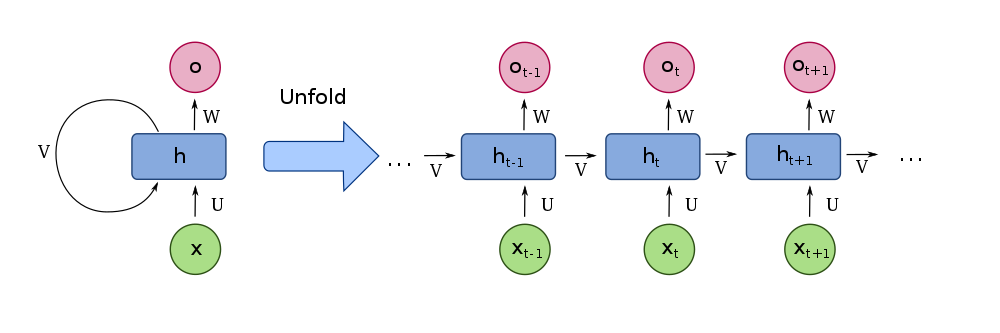
\includegraphics[scale=0.35]{10_deep_learning/02_img/rnn}
	\end{figure}
\end{frame}


% RNN Extensions
\begin{frame}{RNN Extensions}{}\optional
	\begin{itemize}
		\item \textbf{Bi-directionality:} \\
			Run one RNN from left to right and another one from right to left and concatenate the hidden states
			$\overset{\rightarrow}{\bm{h}_t}$ and $\overset{\leftarrow}{\bm{h}_t}$
		\item \textbf{Gating:} \\
			\highlight{Gated Recurrent Units (GRUs)} and \highlight{Long-Short Term Memory (LSTM)} networks modify the recurrent unit
			to better control what is stored in the hidden state $h$ and to prevent a vanishing gradient
		\item \textbf{Skip-connections} through time
	\end{itemize}
\end{frame}


% Inside an LSTM
\begin{frame}{Inside an LSTM [Hochreiter/Schmidhuber, 1997]}{}\optional
	\divideTwo{0.49}{
		\vspace*{3mm}
		\begin{figure}
	\centering
		\begin{tikzpicture}[
			scale=0.5,
			every node/.style={scale=0.5},
			layer/.style={thick,rectangle,draw=black,fill=yellow,minimum height=6mm,minimum width=10mm},
			op/.style={thick,ellipse,draw=black,fill=red!30,minimum width=14mm},
			arr/.style={-stealth,thick},
			edg/.style={thick}
		]

			% cell boundaries
			\draw[very thick,rounded corners,fill=lightgray] (-5,-3) rectangle (6,3);
			
			% input
			\node[circle,thick,draw=black,fill=myblue2] (X) at (-4.5,-5) {$\bm{x_t}$};
			% output
			\node[circle,thick,draw=black,fill=myblue2] (H) at (5.5,5) {$\bm{h_t}$};
			
			% layers
			\node[layer] (F) at (-4,-1) {$\bm{\sigma}$};
			\node[layer] (I) at (-2,-1) {$\bm{\sigma}$};
			\node[layer] (tanh1) at (0,-1) {$\bm{tanh}$};
			\node[layer] (O) at (2,-1) {$\bm{\sigma}$};
			
			% operations
			\node[op] (OpCmF) at (-4,2) {$\bm{\odot}$};
			\node[op] (OpCpI) at (0,2) {$\bm{\oplus}$};
			\node[op] (OpImTanh) at (0,0) {$\bm{\odot}$};
			\node[op] (OpOmTanh) at (4,0) {$\bm{\odot}$};
			\node[op] (OpTanh) at (4,1.25) {\footnotesize $\bm{tanh}$};
			
			% connections
			\draw[arr] (-5,2) -- (OpCmF) -- (OpCpI) -- (7,2);
			\draw[edg] (X) -- (-4.5,-2);
			\draw[arr] (-5,-2) -- ++(7,0) -- (O) -- ++(0,1) -- (OpOmTanh);
			\draw[arr] (-4,-2) -- (F) -- (OpCmF);
			\draw[arr] (-2,-2) -- (I) -- ++(0,1) -- (OpImTanh);
			\draw[arr] (0,-2) -- (tanh1) -- (OpImTanh) -- (OpCpI);
			\draw[arr] (4,2) -- (OpTanh) -- (OpOmTanh) -- ++(0,-2) -- ++(3,0);
			\intersect{5.5,-2}{H}{-5,2}{7,2}{arr};
			\node at (1,-4) {\large Image taken from
				\href{http://colah.github.io/posts/2015-08-Understanding-LSTMs/}{\linkstyle{colah's blog}} (adapted)};

		\end{tikzpicture}
\end{figure}
	}{0.49}{
		\vspace*{-5mm}
		\footnotesize
		\begin{align*}
			\shortintertext{\highlight{Forget gate}}
			\bm{f}_t 				&= \sigma(\bm{\Theta}_f \cdot [\bm{h}_{t-1}, \bm{x}_t] + b_f) 			\\
			\shortintertext{\highlight{Input gate}}
			\bm{i}_t 				&= \sigma(\bm{\Theta}_i \cdot [\bm{h}_{t-1}, \bm{x}_t] + b_i) 			\\
			\widetilde{\bm{C}}_t 		&= \text{tanh}(\bm{\Theta}_C \cdot [\bm{h}_{t-1}, \bm{x}_t] + b_C) 		\\
			\bm{C}_t 				&= \bm{f}_t \odot \bm{C}_{t-1} + \bm{i}_t \odot \widetilde{\bm{C}}_t 		\\
			\shortintertext{\highlight{Output gate}}
			\bm{o}_t 				&= \sigma(\bm{\Theta}_o \cdot [\bm{h}_{t-1}, \bm{x}_t] + b_o) 			\\
			\bm{h}_t 				&= \bm{o}_t \odot \text{tanh}(\bm{C}_t)
		\end{align*}
	}
\end{frame}


% Subsection: Use Cases
% --------------------------------------------------------------------------------------------------------
\subsection{Use Cases}

% Use Case: Neural artistic Style Transfer
\begin{frame}{Use Case: Neural artistic Style Transfer}{}
	\begin{figure}
		\centering
		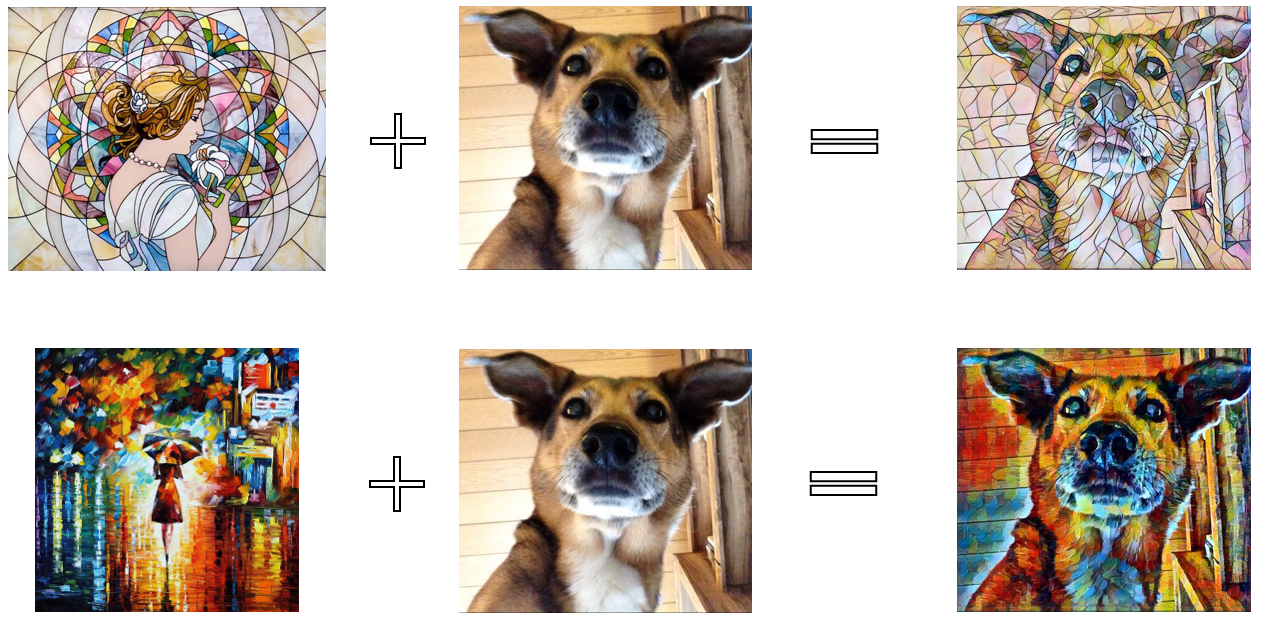
\includegraphics[scale=0.3]{10_deep_learning/02_img/neural_artistic_style_transfer}
	\end{figure}
\end{frame}


% Use Case: Image Generation (GAN)
\begin{frame}{Use Case: Image Generation (GAN)}{}
	\begin{figure}
		\centering
		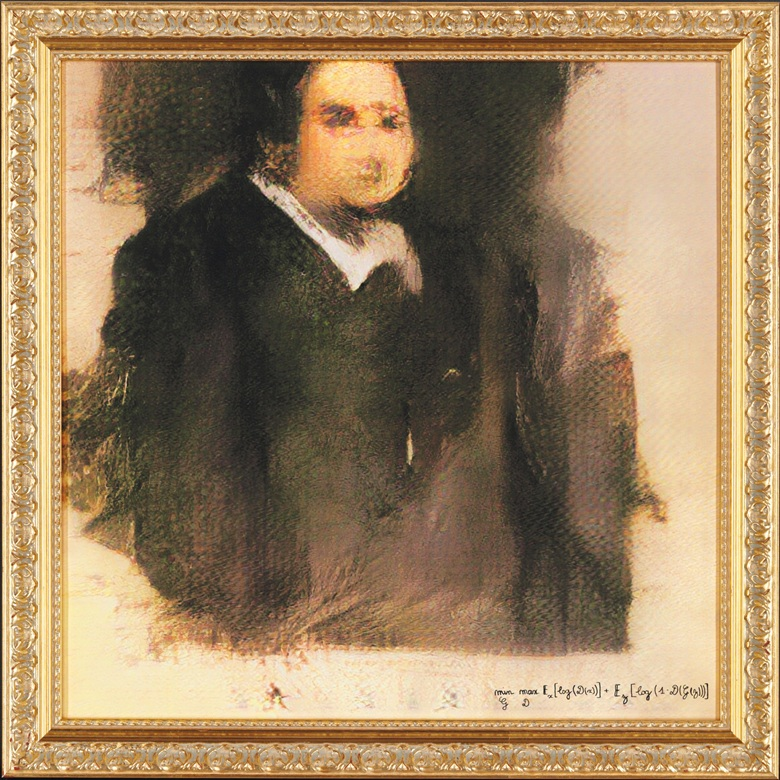
\includegraphics[scale=0.25]{10_deep_learning/02_img/image_generation}
	\end{figure}
\end{frame}


% Use Case: Watermark Removal
\begin{frame}{Use Case: Watermark Removal}{}
	\begin{figure}
		\centering
		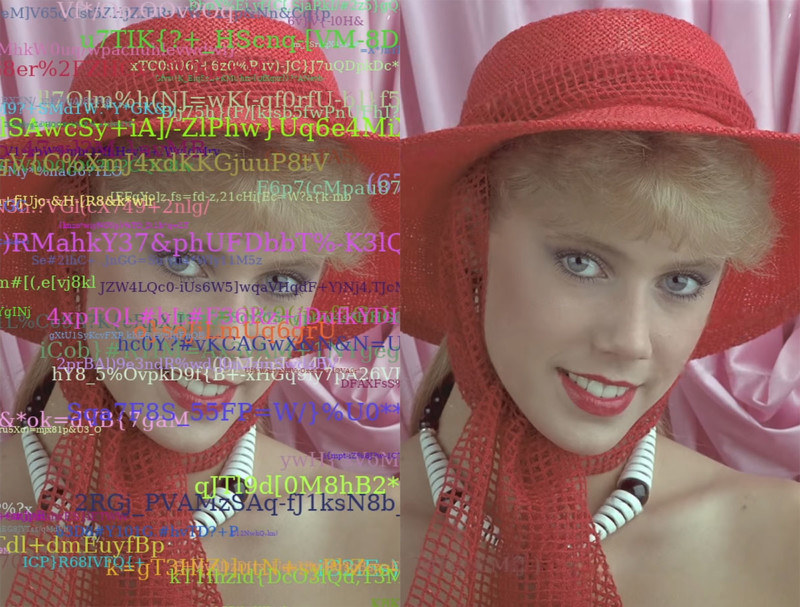
\includegraphics[scale=0.25]{10_deep_learning/02_img/watermark_removal}
	\end{figure}
\end{frame}


% Use Case: Face Recognition
\begin{frame}{Use Case: Face Recognition}{}
	\begin{figure}
		\centering
		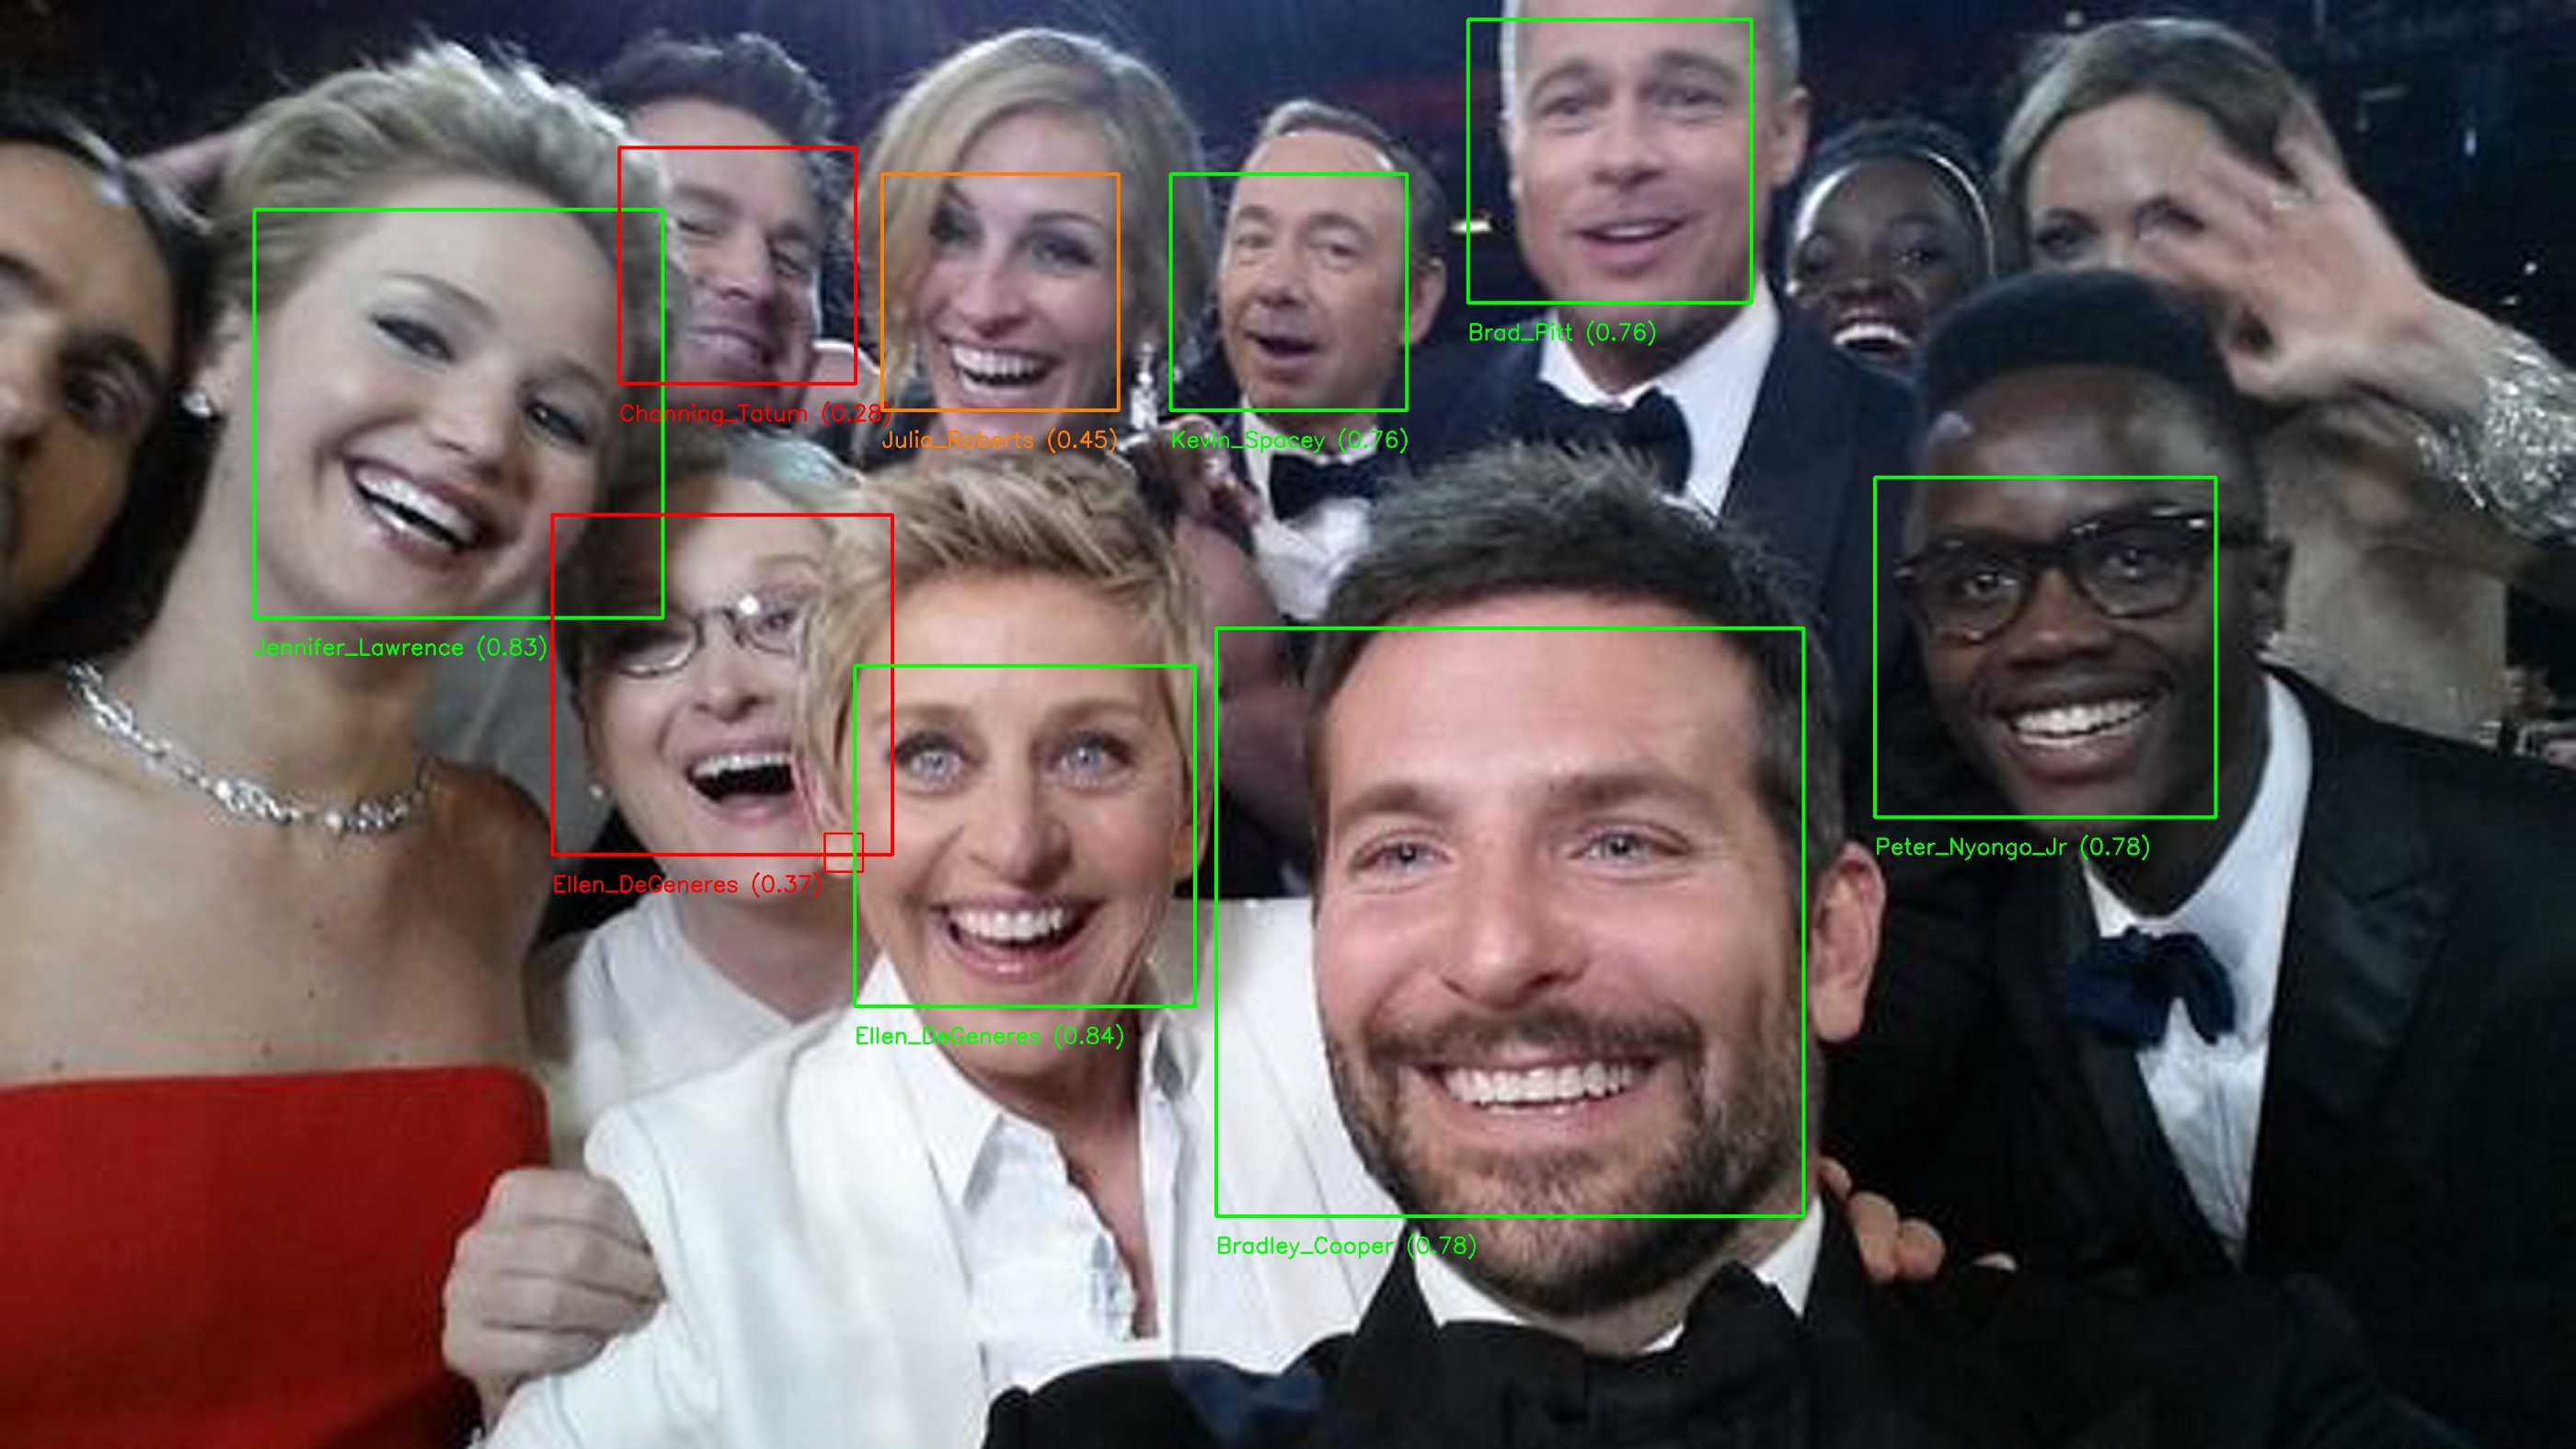
\includegraphics[scale=0.10]{10_deep_learning/02_img/face_recognition}
	\end{figure}
\end{frame}


% Use Case: Meme Generation (seriously...)
\begin{frame}{Use Case: Meme Generation (seriously...)}{}
	\begin{figure}
		\centering
		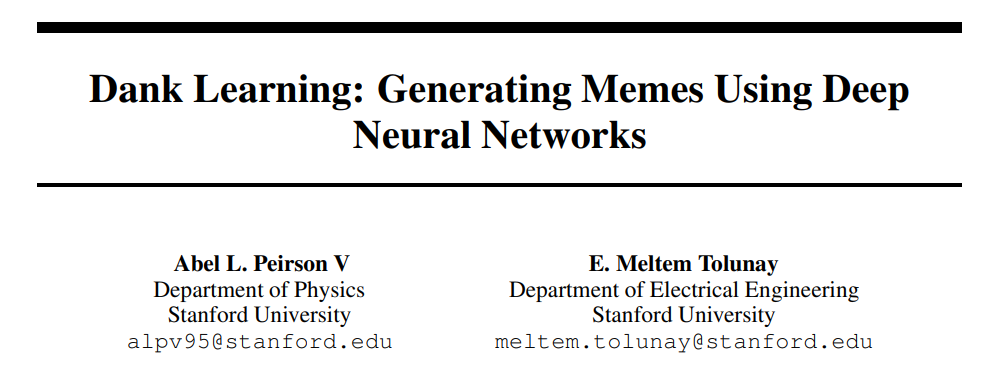
\includegraphics[scale=0.50]{10_deep_learning/02_img/meme_generation}
	\end{figure}
\end{frame}


% Subsection: Word Embeddings
% --------------------------------------------------------------------------------------------------------
\subsection{Word Embeddings}

% Why Vector Representations of natural Language?
\begin{frame}{Why Vector Representations of natural Language?}{}
	\begin{itemize}
		\item \textbf{Why?}
		\begin{itemize}
			\item Most machine learning algorithms (e.\,g. neural nets) cannot handle text input
			\item Therefore, a numeric representation has to be devised
		\end{itemize}
		\item{\textbf{How? -- First ideas:}}
		\begin{itemize}
			\item Strawman idea: Represent each word $w \in \mathcal{V}$ as a one-hot vector
			\item E.\,g. $\mathcal{V} = \{$this, great, be$\}$:
			\begin{equation*}	
				\bm{v}_{\text{this}} = [1,0,0]^{\intercal} \qquad
				\bm{v}_{\text{great}} = [0,1,0]^{\intercal} \qquad
				\bm{v}_{\text{be}} = [0,0,1]^{\intercal}
			\end{equation*}
			\item \textcolor{red}{\textbf{Problems:}} $\bm{v}_{w_i} \in \textcolor{red}{\mathbb{R}^{\vert \mathcal{V} \vert}}$
			 	and semantics are not modeled
		\end{itemize}
	\end{itemize}
\end{frame}


% Distributional Hypothesis [Harris, 1954] and [Firth, 1957]
\begin{frame}{Distributional Hypothesis [Harris, 1954] and [Firth, 1957]}{}
	\begin{itemize}
		\item Other approaches are based onto the \highlight{distributional hypothesis}:
		\begin{itemize}
			\item{} [Harris, 1954]: Words are similar if they occur in similar contexts:
			\vspace*{2mm}
			\begin{center}
				\textit{`The fact that, for example, not every adjective occurs with every noun can be used as a measure
				of meaning  difference. (...) In other words, difference in meaning correlates with difference in distribution.'}
			\end{center}
			\vspace*{2mm}
			\item{} [Firth, 1957]:
			\vspace*{2mm}
			\begin{center}
				\textit{`You shall know a word by the company it keeps.'}
			\end{center}
			\vspace*{2mm}
		\end{itemize}
		\item It is possible to represent words by its context! Such models are called \highlight{count models}
			[Baroni et al., 2014]
	\end{itemize}
\end{frame}


% Distributional Hypothesis (Ctd.)
\begin{frame}{Distributional Hypothesis (Ctd.)}{}
	\begin{itemize}
		\item Famous example by [McDonald and Ramscar, 2001]:
		\vspace*{2mm}
		\begin{center}
			\textit{He filled the \textbf{wampimuk}, passed it around and we all drank some.} \\
			$\Rightarrow$ jar, cup, glass, ...
		\end{center}
		\vspace*{2mm}
		\pause
		\begin{center}
			\textit{We found a little hairy \textbf{wampimuk} sleeping behind the tree.} \\
			$\Rightarrow$ cat, bear, raccoon, ...
		\end{center}
		\vspace*{2mm}
		\item \highlight{Based on the context the invented word \underline{`wampimuk'} is associated with a different meaning}
	\end{itemize}
\end{frame}


% Count Models
\begin{frame}{Count Models}{}
	\begin{itemize}
		\item Set a window size $m$ and count \# of times a word occurs in that window
		\item We get a $\vert \mathcal{V} \vert \times \vert \mathcal{V} \vert$ count matrix $\bm{M}$
		\item Similar approach: \highlight{Latent semantic analysis} [Deerwester et al., 1990]
	\end{itemize}
	\divideTwo{0.39}{
		\vspace*{-3mm}
		Example by R. Socher:
		\begin{itemize}
			\item I like deep learning .
			\item I like NLP .
			\item I enjoy flying .
		\end{itemize}
	}{0.59}{
		\vspace*{4mm}
		\begin{table}
	\renewcommand{\arraystretch}{0.9}
	\scalebox{0.6}{
	\begin{tabular}{| c || c | c | c | c | c | c | c | c |}
		\hline
		\multicolumn{9}{| c |}{\textbf{Window size: $m = 1$}} \\ \hline
		\textbf{Counts} &
		\textbf{I} &
		\textbf{like} &
		\textbf{enjoy} &
		\textbf{deep} &
		\textbf{learning} &
		\textbf{NLP} &
		\textbf{flying} &
		\textbf{.}
		\\ \hline\hline
		\textbf{I} 			& 0 & 2 & 1 & 0 & 0 & 0 & 0 & 0 \\ \hline
		\textbf{like} 		& 2 & 0 & 0 & 1 & 0 & 1 & 0 & 0 \\ \hline
		\textbf{enjoy} 		& 1 & 0 & 0 & 0 & 0 & 0 & 1 & 0 \\ \hline
		\textbf{deep} 		& 0 & 1 & 0 & 0 & 1 & 0 & 0 & 0 \\ \hline
		\textbf{learning} 	& 0 & 0 & 0 & 1 & 0 & 0 & 0 & 1 \\ \hline
		\textbf{NLP}		& 0 & 1 & 0 & 0 & 0 & 0 & 0 & 1 \\ \hline
		\textbf{flying} 		& 0 & 0 & 1 & 0 & 0 & 0 & 0 & 1 \\ \hline
		\textbf{.}			& 0 & 0 & 0 & 0 & 1 & 1 & 1 & 0 \\ \hline
	\end{tabular}}		
\end{table}
	}
\end{frame}


% Count Models (Ctd.)
\begin{frame}{Count Models (Ctd.)}{}
	\begin{itemize}
		\item Each column (or row) can be used as a word vector
		\item \textbf{Observations:}
		\begin{enumerate}
			\item Due to the counts the word vector now captures the context/semantics better
			\item The vector is still huge! (size of the vocabulary)
		\end{enumerate}
		\item \highlight{Singular value decomposition (SVD)} is performed in order to reduce the dimensionality of the
			matrix $\bm{M}$:
		\begin{equation*}
			\bm{M} = \bm{U} \bm{\Sigma} \bm{V}^{\intercal}
		\end{equation*}
		\item We can now use matrix $\bm{U}$ as a reduced version
	\end{itemize}
\end{frame}


% word2vec
\begin{frame}{word2vec [Mikolov et al., 2013]}{}
	\begin{itemize}
		\item Why not learning compact word representations in the first place?
		\item T. Mikolov et al. proposed \highlight{word2vec}
		\item \textbf{Unsupervised learning} using an \textbf{auxiliary task}
		\item The auxiliary task is inspired by the concept of \highlight{language models}, \\ e.\,g. [Bengio et al., 2003]
		\begin{itemize}
			\item A language model predicts the next word given the previous words
			\item E.\,g.: \textit{A dog is a man's best} $\rule{2cm}{0.15mm}$ .
		\end{itemize} 
	\end{itemize}
\end{frame}


% CBOW vs. Skip-Gram
\begin{frame}{CBOW vs. Skip-Gram}{}
	\textbf{Mikolov et al. propose two architectures:} \vspace*{2mm}
	\begin{itemize}
		\item \highlight{CBOW (Continuous bag-of-words):} \\
			Predict the middle word given the context, e.\,g.:
		\vspace*{2mm}
		\begin{center}
			same procedure $\rule{2cm}{0.15mm}$ every year
		\end{center}
		\vspace*{2mm}
		\item \highlight{Skip-Gram:} \\
			Predict the context words given the middle word, e.\,g.:
		\vspace*{2mm}
		\begin{center}
			$\rule{2cm}{0.15mm}$ $\rule{2cm}{0.15mm}$ as $\rule{2cm}{0.15mm}$ $\rule{2cm}{0.15mm}$
		\end{center}
	\end{itemize}
\end{frame}


% CBOW vs. Skip-Gram (Ctd.)
\begin{frame}{CBOW vs. Skip-Gram (Ctd.)}{}
	\divideTwo{0.49}{
		\begin{figure}
	\centering
	\begin{tikzpicture}[
		scale=0.4,
		every node/.style={scale=0.6},
		n/.style={circle,draw=black,thick,minimum width=1cm},
		arr/.style={-stealth,thick}
	]

		\node[rotate=90] at (-6,0) {\highlight{\large CBOW}};

		% input
		\node at (-3,7) {\textbf{Input}};
		\node[n] (I1) at (-3,5) {$\bm{w}_{t-2}$}; 
		\node[n] (I2) at (-3,2.5) {$\bm{w}_{t-1}$};
		\node[n] (I3) at (-3,-2.5) {$\bm{w}_{t+1}$}; 
		\node[n] (I4) at (-3,-5) {$\bm{w}_{t+2}$};
		
		% projection
		\node at (0,7) {\textbf{Projection}};
		\node[n] (P1) at (0,0) {};
		
		% output
		\node at (3,7) {\textbf{Output}};
		\node[n] (O1) at (3,0) {$\bm{w}_t$};

		% connections
		\draw[arr] (I1) -- (P1); \draw[arr] (I2) -- (P1); \draw[arr] (I3) -- (P1); \draw[arr] (I4) -- (P1);
		\draw[arr] (P1) -- (O1);

	\end{tikzpicture}
\end{figure}
	}{0.49}{
		\begin{figure}
	\centering
	\begin{tikzpicture}[
		scale=0.4,
		every node/.style={scale=0.6},
		n/.style={circle,draw=black,thick,minimum width=1cm},
		arr/.style={-stealth,thick}
	]

		\node[rotate=90] at (6,0) {\highlight{\large Skip-Gram}};
		
		% input
		\node at (-3,7) {\textbf{Input}};
		\node[n] (I1) at (-3,0) {$\bm{w}_t$};
	

		% projection
		\node at (0,7) {\textbf{Projection}};
		\node[n] (P1) at (0,0) {};

		% output
		\node at (3,7) {\textbf{Output}};
		\node[n] (O1) at (3,5) {$\bm{w}_{t-2}$}; 
		\node[n] (O2) at (3,2.5) {$\bm{w}_{t-1}$};
		\node[n] (O3) at (3,-2.5) {$\bm{w}_{t+1}$}; 
		\node[n] (O4) at (3,-5) {$\bm{w}_{t+2}$};
		
		% connections
		\draw[arr] (I1) -- (P1);
		\draw[arr] (P1) -- (O1); \draw[arr] (P1) -- (O2); \draw[arr] (P1) -- (O3); \draw[arr] (P1) -- (O4);

	\end{tikzpicture}
\end{figure}
	}
\end{frame}


% Skip-Gram in more Detail
\begin{frame}{Skip-Gram in more Detail}{}
	\divideTwo{0.49}{
		\begin{figure}
	\centering
	\begin{tikzpicture}[
		scale=0.4,
		every node/.style={scale=0.6},
		n/.style={circle,draw=black,thick,minimum width=1cm},
		arr/.style={-stealth,thick}
	]

		\node[rotate=90] at (6,0) {\highlight{\large Skip-Gram}};
		
		% input
		\node at (-3,7) {\textbf{Input}};
		\node[n] (I1) at (-3,0) {$\bm{w}_t$};
	

		% projection
		\node at (0,7) {\textbf{Projection}};
		\node[n] (P1) at (0,0) {};

		% output
		\node at (3,7) {\textbf{Output}};
		\node[n] (O1) at (3,5) {$\bm{w}_{t-2}$}; 
		\node[n] (O2) at (3,2.5) {$\bm{w}_{t-1}$};
		\node[n] (O3) at (3,-2.5) {$\bm{w}_{t+1}$}; 
		\node[n] (O4) at (3,-5) {$\bm{w}_{t+2}$};
		
		% connections
		\draw[arr] (I1) -- (P1);
		\draw[arr] (P1) -- (O1); \draw[arr] (P1) -- (O2); \draw[arr] (P1) -- (O3); \draw[arr] (P1) -- (O4);

		\node at (-1.5,1) {$\bm{E}$};

	\end{tikzpicture}
\end{figure}
	}{0.49}{
		\begin{itemize}
			\item The input/labels are \textbf{one-hot vectors} (also for CBOW)
			\item $\bm{E} \in \mathbb{R}^{d \times \vert \mathcal{V} \vert}$ is a \textbf{shared embedding matrix}
			\item \textbf{Identity activation} in the projection layer
			\item $\bm{w} \bm{E} = \bm{v} \in \mathbb{R}^{d \times 1}$ is the embedding of word $\bm{w}$
				(since $\bm{w}$ is one-hot)
		\end{itemize}
	}
\end{frame}


% Skip-Gram in more Detail (Ctd.)
\begin{frame}[plain]{}{}
	\begin{figure}
	\centering
	\begin{tikzpicture}[
		scale=0.3,
		every node/.style={scale=0.55},
		box/.style={rounded corners,dashed}
	]

		\node[rotate=90] at (37,0) {\highlight{context words}};
		\node at (4,-13) {Image taken from Manning (adapted): \url{https://www.youtube.com/watch?v=ERibwqs9p38}};

		\draw[box,fill=lightgray!10] (-11,-12) rectangle (-5,14);
		\draw[box,fill=lightgray!20] (-3,-12) rectangle (7,14);
		\draw[box,fill=lightgray!30] (9,-12) rectangle (15,14);

		\node[align=center] at (-8,12) {$\vert \mathcal{V} \vert \times 1$ \\ $w_t$};
		\node[align=center] at (-8,-8) {\highlight{One-hot} \\ \highlight{word vector} \\ \highlight{center word}};

		\node[align=center] at (2,12) {$d \times \vert \mathcal{V} \vert$ \\ $\bm{E}$};
		\node[align=center] at (2,-8) {\highlight{Word embedding matrix}};

		\node[align=center] at (12,12) {$d \times 1$ \\ $\bm{v}_c$};
		\node[align=center] at (12,-8) {\highlight{Word emb.} \\ \highlight{for center word}};

		\node[align=center] at (19,14) {$\vert \mathcal{V} \vert \times d$ \\ $\bm{U}$};
		\node[align=center] at (25,14) {$\vert \mathcal{V} \vert \times 1$ \\ $\bm{u}_o^{\intercal} \bm{v}_c$};
		\node[align=center] at (30,14) {$\vert \mathcal{V} \vert \times 1$ \\ soft-max};
		\node[align=center] at (35,14) {$\vert \mathcal{V} \vert \times 1$ \\ truth};

		\node at (-4,0) {\Large $\times$};
		\node at (8,0) {\Large $=$};

		\node at (-8,0) {$\begin{bmatrix} 0 \\ 0 \\ 0 \\ 0 \\ 0 \\ 1 \\ 0 \\ 0 \\ 0 \end{bmatrix}$};
		\node at (2,0) {$
			\begin{bmatrix*}[r]
				\bullet 	& \hdots 	& 0.2 	& \hdots & \bullet \\[3.2mm]
				\bullet 	& \hdots 	& -1.4 	& \hdots & \bullet \\[3.2mm]
				\bullet 	& \hdots 	& 0.3 	& \hdots & \bullet \\[3.2mm]
				\bullet 	& \hdots 	& -0.1 	& \hdots & \bullet \\[3.2mm]
				\bullet 	& \hdots 	& 0.1 	& \hdots & \bullet \\[3.2mm]
				\bullet 	& \hdots 	& 0.5 	& \hdots & \bullet
			\end{bmatrix*}$};
		\node at (12,0) {$
			\begin{bmatrix*}[r]
				0.2 	\\[3.2mm]
				-1.4	\\[3.2mm]
				0.3 	\\[3.2mm]
				-0.1	\\[3.2mm]
				0.1 	\\[3.2mm]
				0.5
			\end{bmatrix*}$};

			\draw[thick] (16,-3.5) rectangle (22,3.7);
			\draw[thick] (16,-3.5) -- (22,5) -- (22,12.2) -- (16,3.7);
			\draw[thick] (16,3.7) -- (22,-5) -- (22,-12.2) -- (16,-3.5);

		\node at (25,8.75) {$
			\begin{bmatrix*}[r]
				0.2 		\\[3.2mm]
				0.3		\\[3.2mm]
				0.1 		\\[3.2mm]
				\vdots 	\\[3.2mm]
				0.7
			\end{bmatrix*}$};

		\node at (30,8.75) {$
			\begin{bmatrix*}[r]
				0.08 	\\[3.2mm]
				0.10	\\[3.2mm]
				0.05 	\\[3.2mm]
				\vdots 	\\[3.2mm]
				\textcolor{myblue1}{0.65}
			\end{bmatrix*}$};
			\node at (35,8.75) {$\begin{bmatrix} 0 \\[3.2mm] 0 \\[3.2mm] 0 \\[3.2mm] \vdots \\[3.2mm] \textcolor{myblue1}{1} \end{bmatrix}$};
			
		\node at (25,0.1) {$
			\begin{bmatrix*}[r]
				0.7 		\\[3.2mm]
				0.3		\\[3.2mm]
				0.1 		\\[3.2mm]
				\vdots 	\\[3.2mm]
				-0.1
			\end{bmatrix*}$};

		\node at (30,0.1) {$
			\begin{bmatrix*}[r]
				\textcolor{myblue1}{0.65} 	\\[3.2mm]
				0.10	\\[3.2mm]
				0.05 	\\[3.2mm]
				\vdots 	\\[3.2mm]
				0.03
			\end{bmatrix*}$};
			\node at (35,0.1) {$\begin{bmatrix} 0 \\[3.2mm] \textcolor{myblue1}{1} \\[3.2mm] 0 \\[3.2mm] \vdots \\[3.2mm] 0 \end{bmatrix}$};

		\node at (25,-8.75) {$
			\begin{bmatrix*}[r]
				0.5 		\\[3.2mm]
				0.7		\\[3.2mm]
				0.1		\\[3.2mm]
				\vdots 	\\[3.2mm]
				0.4
			\end{bmatrix*}$};

		\node at (30,-8.75) {$
			\begin{bmatrix*}[r]
				\textcolor{myblue1}{0.40} 	\\[3.2mm]
				0.15	\\[3.2mm]
				0.05 	\\[3.2mm]
				\vdots 	\\[3.2mm]
				0.30
			\end{bmatrix*}$};
			\node at (35,-8.75) {$\begin{bmatrix} 0 \\[3.2mm] 0 \\[3.2mm] 0 \\[3.2mm] \vdots \\[3.2mm] \textcolor{myblue1}{1} \end{bmatrix}$};

	\end{tikzpicture}
\end{figure}
\end{frame}


% Skip-Gram Training Objective
\begin{frame}{Skip-Gram Training Objective}{}
	\begin{itemize}
		\item Skip-Gram optimizes the \highlight{negative log-likelihood}:
		\begin{equation*}
			\footnotesize
			\mathcal{J}(\bm{\theta}) = -\frac{1}{T} \sum_{t=1}^T \sum_{\substack{-m \le j \le m\\ j \ne 0}}
				\log p(w_{t+j} \vert w_t; \bm{\theta})
		\end{equation*}
		\item The probability is given by the soft-max:
		\begin{equation*}
			\footnotesize
			p(o \vert c) = \frac{\exp\{ \bm{u}_o^{\intercal} \bm{v}_c \}}{
				\sum_{w=1}^{\vert \mathcal{V} \vert} \exp\{ \bm{u}_w^{\intercal} \bm{v}_c \}}
		\end{equation*}
		\item $t$ is the index into the corpus, $o$ and $c$ are indices into the vocabulary
	\end{itemize}
\end{frame}


% Evaluation of Word Embeddings
\begin{frame}{Evaluation of Word Embeddings}{}
	\begin{itemize}
		\item As Mikolov et al. found out, the embeddings do not only capture \textbf{syntactic regularities}...
		\item ...but also \textbf{semantic aspects} of the words
		\item \textbf{How did the authors get this insight?}
		\item[$\bm{\Rightarrow}$] Definition of a set of 9 syntactic and 5 semantic questions/tasks, e.\,g.:
		\begin{itemize}
			\item Adjective to adverb (e.\,g. \texttt{bad} $\Leftrightarrow$ \texttt{badly})
			\item Comparative (e.\,g. \texttt{great} $\Leftrightarrow$ \texttt{greater})
			\item Nation adjective (e.\,g. \texttt{France} $\Leftrightarrow$ \texttt{French})
		\end{itemize}
	\end{itemize}
\end{frame}


% Evaluation of Word Embeddings (Ctd.)
\begin{frame}{Evaluation of Word Embeddings (Ctd.)}{}
	\begin{itemize}
		\item An instance of a \underline{syntactic} question (Comparative):
		\vspace*{2mm}
		\begin{center}
			\textit{What is the word that is similar to \textbf{small} in the same sense as \\
			\textbf{biggest} is similar to \textbf{big}?}
		\end{center}
		\vspace*{2mm}
		\item One very famous \underline{semantic} example (Man-Woman):
		\vspace*{2mm}
		\begin{center}
			\textit{\textbf{Man} relates to \textbf{king} like \textbf{woman} does to...?}
		\end{center}
	\end{itemize}
\end{frame}


% Evaluation of Word Embeddings (Ctd.)
\begin{frame}{Evaluation of Word Embeddings (Ctd.)}{}
	\begin{itemize}
		\item Such questions can be answered by performing basic algebraic operations:
		\begin{equation*}
			\bm{v}_{biggest} - \bm{v}_{big} + \bm{v}_{small} \approx \bm{v}_{smallest}
		\end{equation*}
		\begin{equation*}
			\bm{v}_{king} - \bm{v}_{man} + \bm{v}_{woman} \approx \bm{v}_{queen}
		\end{equation*}
		\item A visual example:
		\begin{figure}
	\centering
	\begin{tikzpicture}[
		scale=0.45,
		every node/.style={scale=0.55},
		arr/.style={-stealth,thick}
	]

		\node (M) at (0,0) {Man};
		\node (W) at (2,2) {Woman};
		\draw[arr,blue] (M) -- (W);
		
		\node (U) at (3,0) {Uncle};
		\node (A) at (5,2) {Aunt};
		\draw[arr,blue] (U) -- (A);
		
		\node (K1) at (-0.5,-3) {King};
		\node (Q1) at (1.5,-1) {Queen};
		\draw[arr,blue] (K1) -- (Q1);

		\draw[dashed,thick] (7.5,2) -- (7.5,-3);


		\node (K2) at (12,-3) {King};
		\node (Ks) at (10,0) {Kings};
		\node (Q2) at (14,-1) {Queen};
		\node (Qs) at (12,2) {Queens};

		\draw[arr,red] (K2) -- (Ks);
		\draw[arr,red] (Q2) -- (Qs);
		\draw[arr,blue] (K2) -- (Q2);

	\end{tikzpicture}
\end{figure}
	\end{itemize}
\end{frame}


% Result of Country Capital Task
\begin{frame}{Result of Country Capital Task}{}
	\begin{figure}
		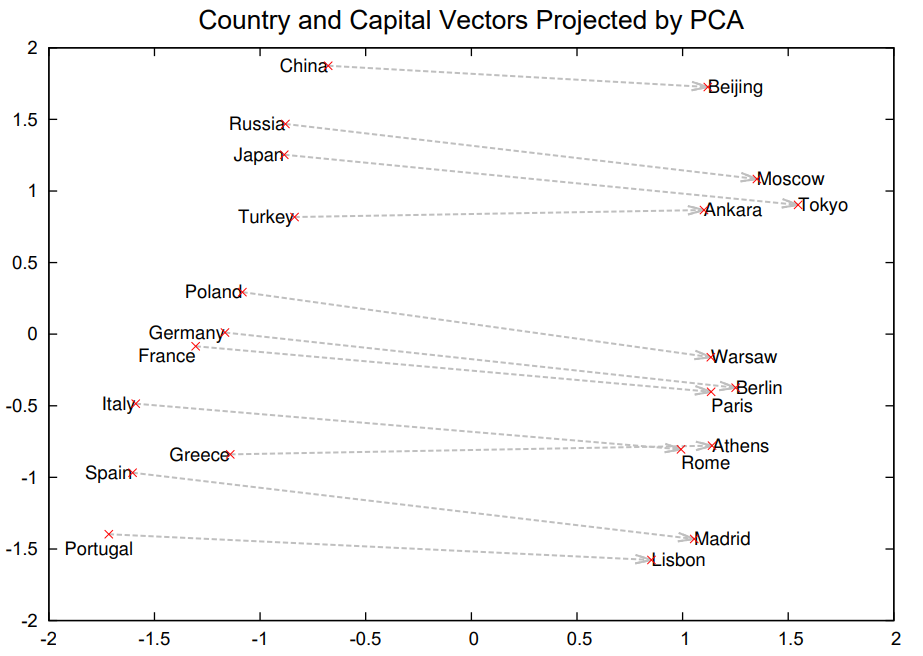
\includegraphics[scale=0.3]{10_deep_learning/02_img/country_capital}
	\end{figure}
\end{frame}


% Section: Wrap-Up
%______________________________________________________________________
\section{Wrap-Up}
\makedivider{Wrap-Up}

% Subsection: Summary
% --------------------------------------------------------------------------------------------------------
\subsection{Summary}

% Summary
\begin{frame}{Summary}{}
	\begin{itemize}
		\item Neural Networks are powerful models for pattern recognition
		\item The perceptron can classify all training examples correctly, \textbf{iff the training data is linearly separable}
		\item \textbf{MLPs are universal function approximators}
		\item Backpropagation is a recursive procedure based on the \textbf{chain rule of calculus} to obtain the gradients for neural network learning
		\item Different neural network architectures like CNNs and RNNs exist for solving different kinds of problems
	\end{itemize}
\end{frame}


% Subsection: Self-Test Questions
% --------------------------------------------------------------------------------------------------------
\subsection{Self-Test Questions}

% Self-Test Questions
\begin{frame}{Self-Test Questions}{}\important
	\begin{enumerate}
		\item What is the relation between neural networks and logistic regression?
		\item What is a perceptron? Which problems can it solve and which not?
		\item Why do we often use multiple layers instead of a simple perceptron?
		\item How does backpropagation work? How does a neural network learn?
		\item What are advantages and disadvantages of using neural networks?
		\item What are CNNs and RNNs? For which tasks are they suitable?
		\item How can words be represented in vectorial form?
	\end{enumerate}
\end{frame}


% Subsection: Lecture Outlook
% --------------------------------------------------------------------------------------------------------
\subsection{Lecture Outlook}

\begin{frame}{What's next...?}{}
	\makeoverview{8}
\end{frame}


% Subsection: Recommended Literature and further Reading
% --------------------------------------------------------------------------------------------------------
\subsection{Recommended Literature and further Reading}

% Literature
%______________________________________________________________________
\begin{frame}[allowframebreaks]{Recommended Literature and further Reading}{}
	\footnotesize
	\begin{thebibliography}{2}
		\literature{book}{Goodfellow.2016}{[1] Deep Learning}
			{Ian Goodfellow et al. MIT Press. 2016.}{$\rightarrow$ \href{
				http://www.deeplearningbook.org/
			}{\linkstyle{Link}}, cf. chapters 6 \textit{Deep Feedforward Networks}, especially chapter 6.5}
	
		\literature{book}{Bishop.2006}{[2] Pattern Recognition and Machine Learning}
			{Christopher Bishop. Springer. 2006.}{$\rightarrow$ \href{
				http://users.isr.ist.utl.pt/~wurmd/Livros/school/Bishop\%20-\%20Pattern\%20Recognition\%20And\%20Machine\%20Learning\%20-\%20Springer\%20\%202006.pdf
			}{\linkstyle{Link}}, cf. chapter 5, especially chapter 5.3}

		\literature{online}{Saunderson.2017}{[3] Backpropagation calculus}
			{Grant Sanderson. YouTube. 2017.}{$\rightarrow$ \href{
				https://www.youtube.com/watch?v=tIeHLnjs5U8
			}{\linkstyle{Link}}}
		\literature{online}{Ng.2019}{[4] Simple Backpropagation in NumPy}
			{Andrew Ng et al. Stanford CS229. 2019.}{$\rightarrow$ \href{
				http://cs229.stanford.edu/notes/backprop.py
			}{\linkstyle{Link}}}
	\end{thebibliography}
\end{frame}


% Subsection: Meme of the Day
% --------------------------------------------------------------------------------------------------------
\subsection{Meme of the Day}

% Meme of the Day
\begin{frame}{Meme of the Day}{}
	\begin{figure}
		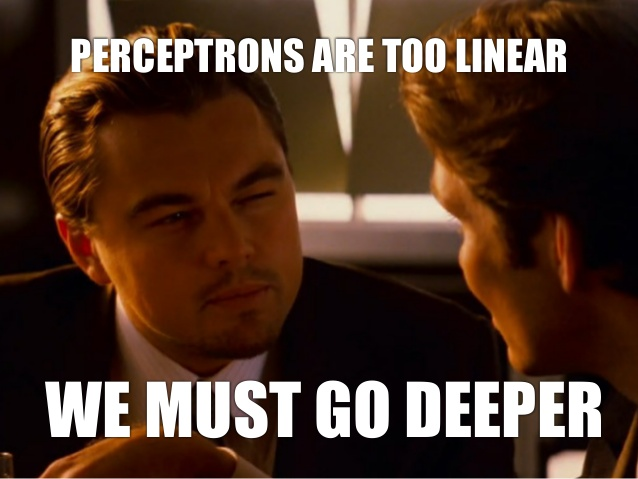
\includegraphics[scale=0.3]{10_deep_learning/02_img/meme_of_the_day}
	\end{figure}
\end{frame}


% Thank you
%______________________________________________________________________
\makethanks

\end{document}